\begin{frame}{Resultados}
  \framesubtitle{Animaciones: experimento y simulación}
  \begin{columns}[T]
    \begin{column}{0.49\textwidth}
      \centering{\small Evento 15 (menor $E^{(2)}_m$)}\par\smallskip
      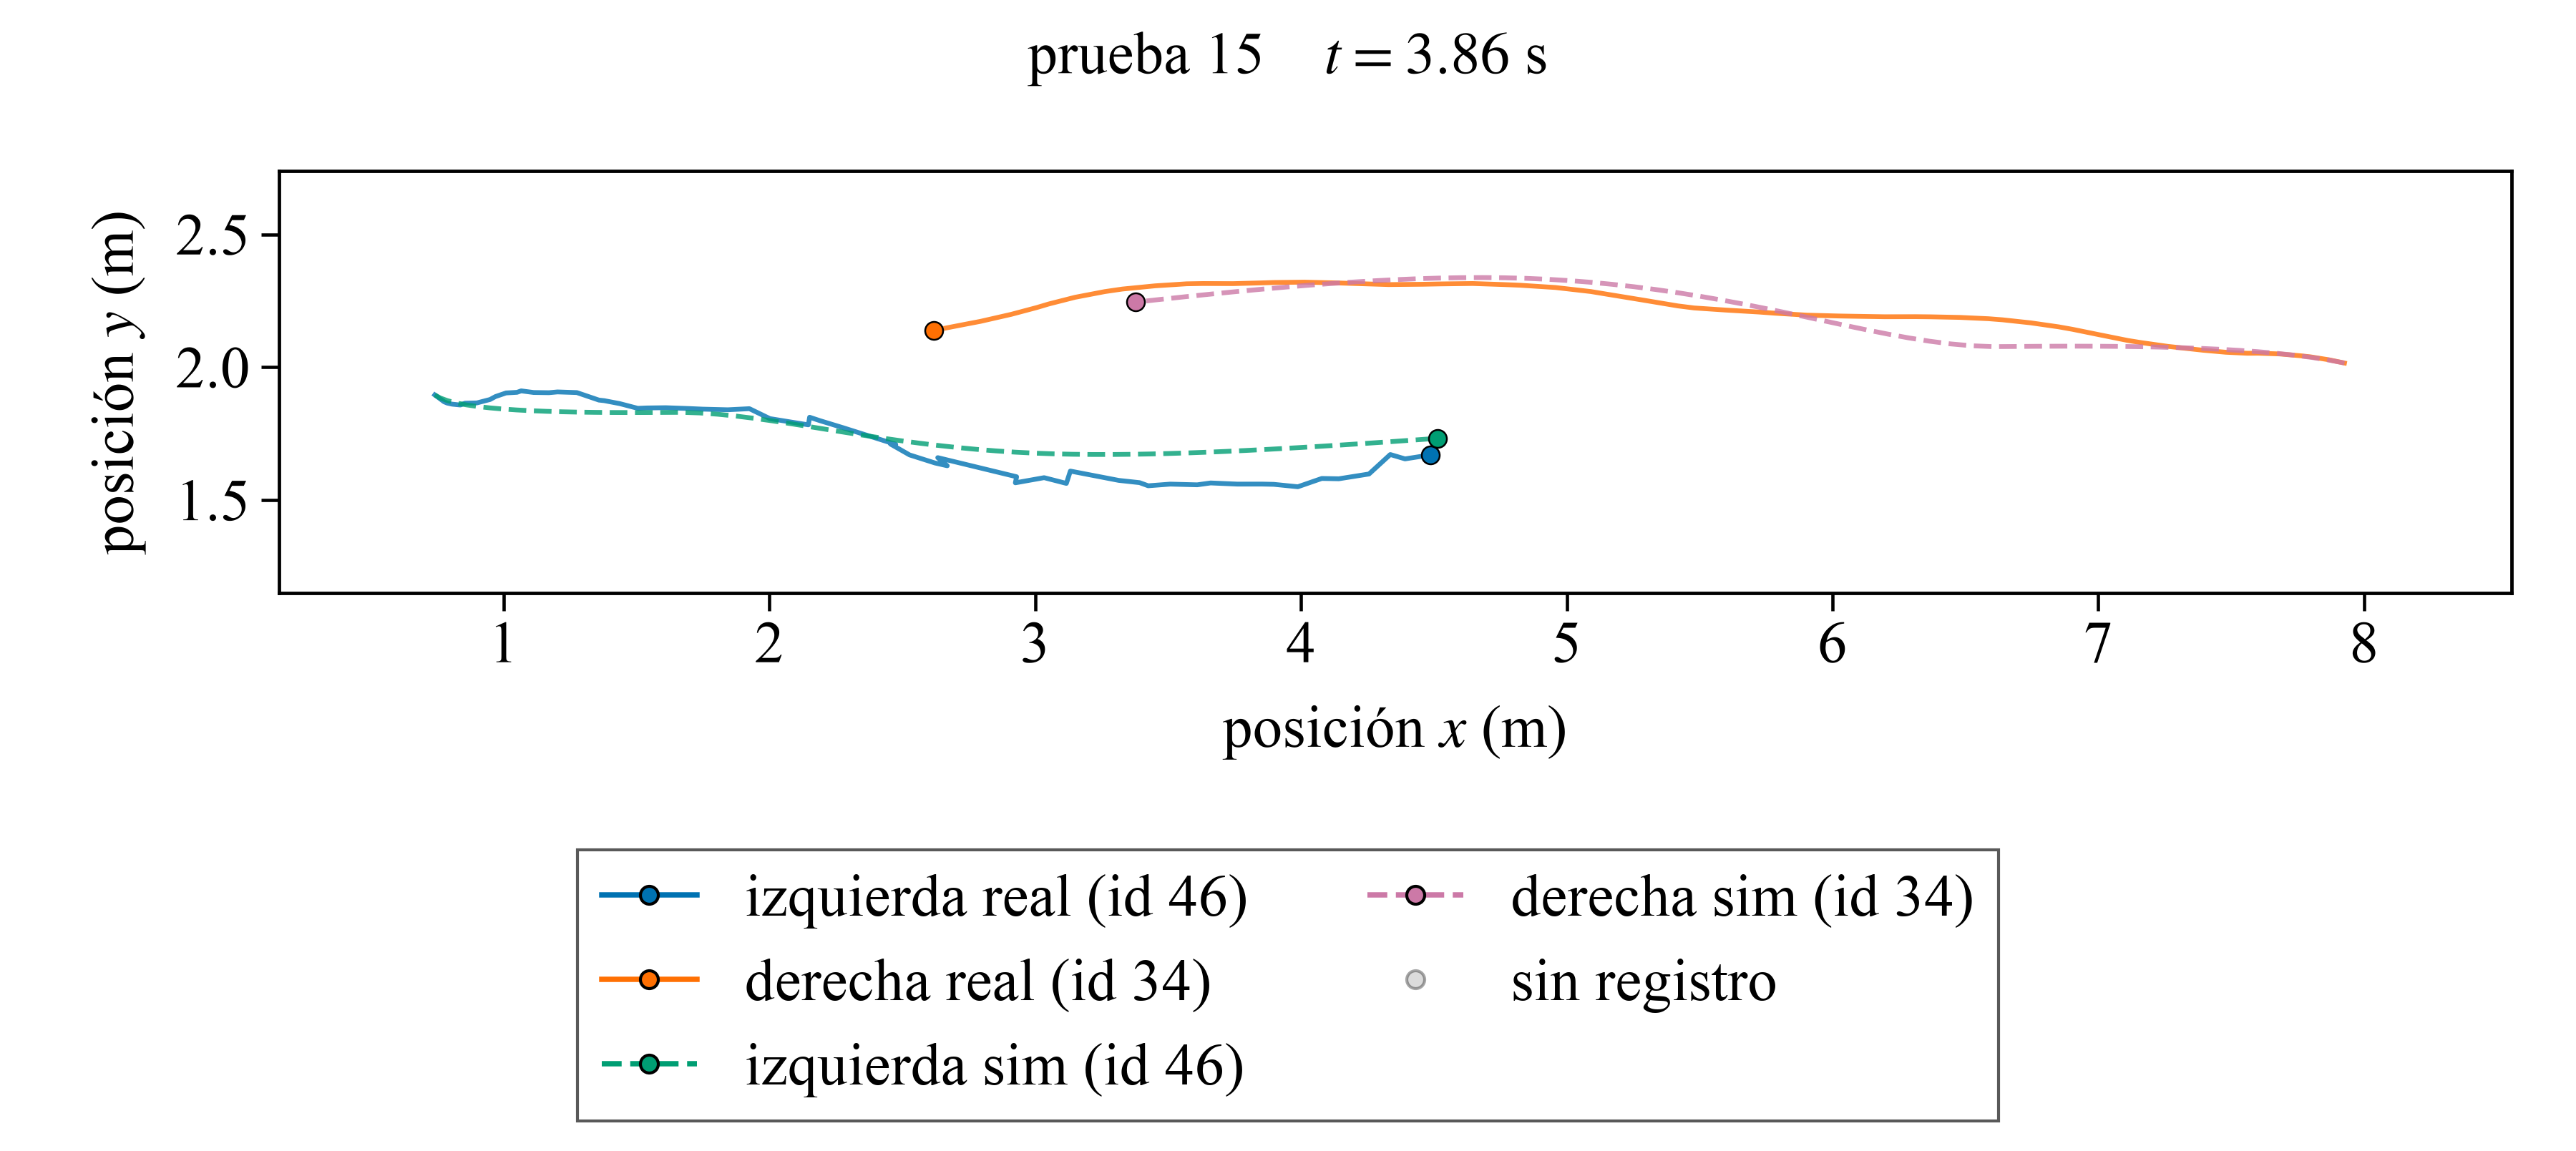
\includegraphics[width=\linewidth,height=0.52\textheight,keepaspectratio]{anim_a.png}
      \par\smallskip{\scriptsize\url{https://youtu.be/PENDIENTE}}
    \end{column}
    \begin{column}{0.49\textwidth}
      \centering{\small Evento 11 (mayor $E^{(2)}_m$)}\par\smallskip
      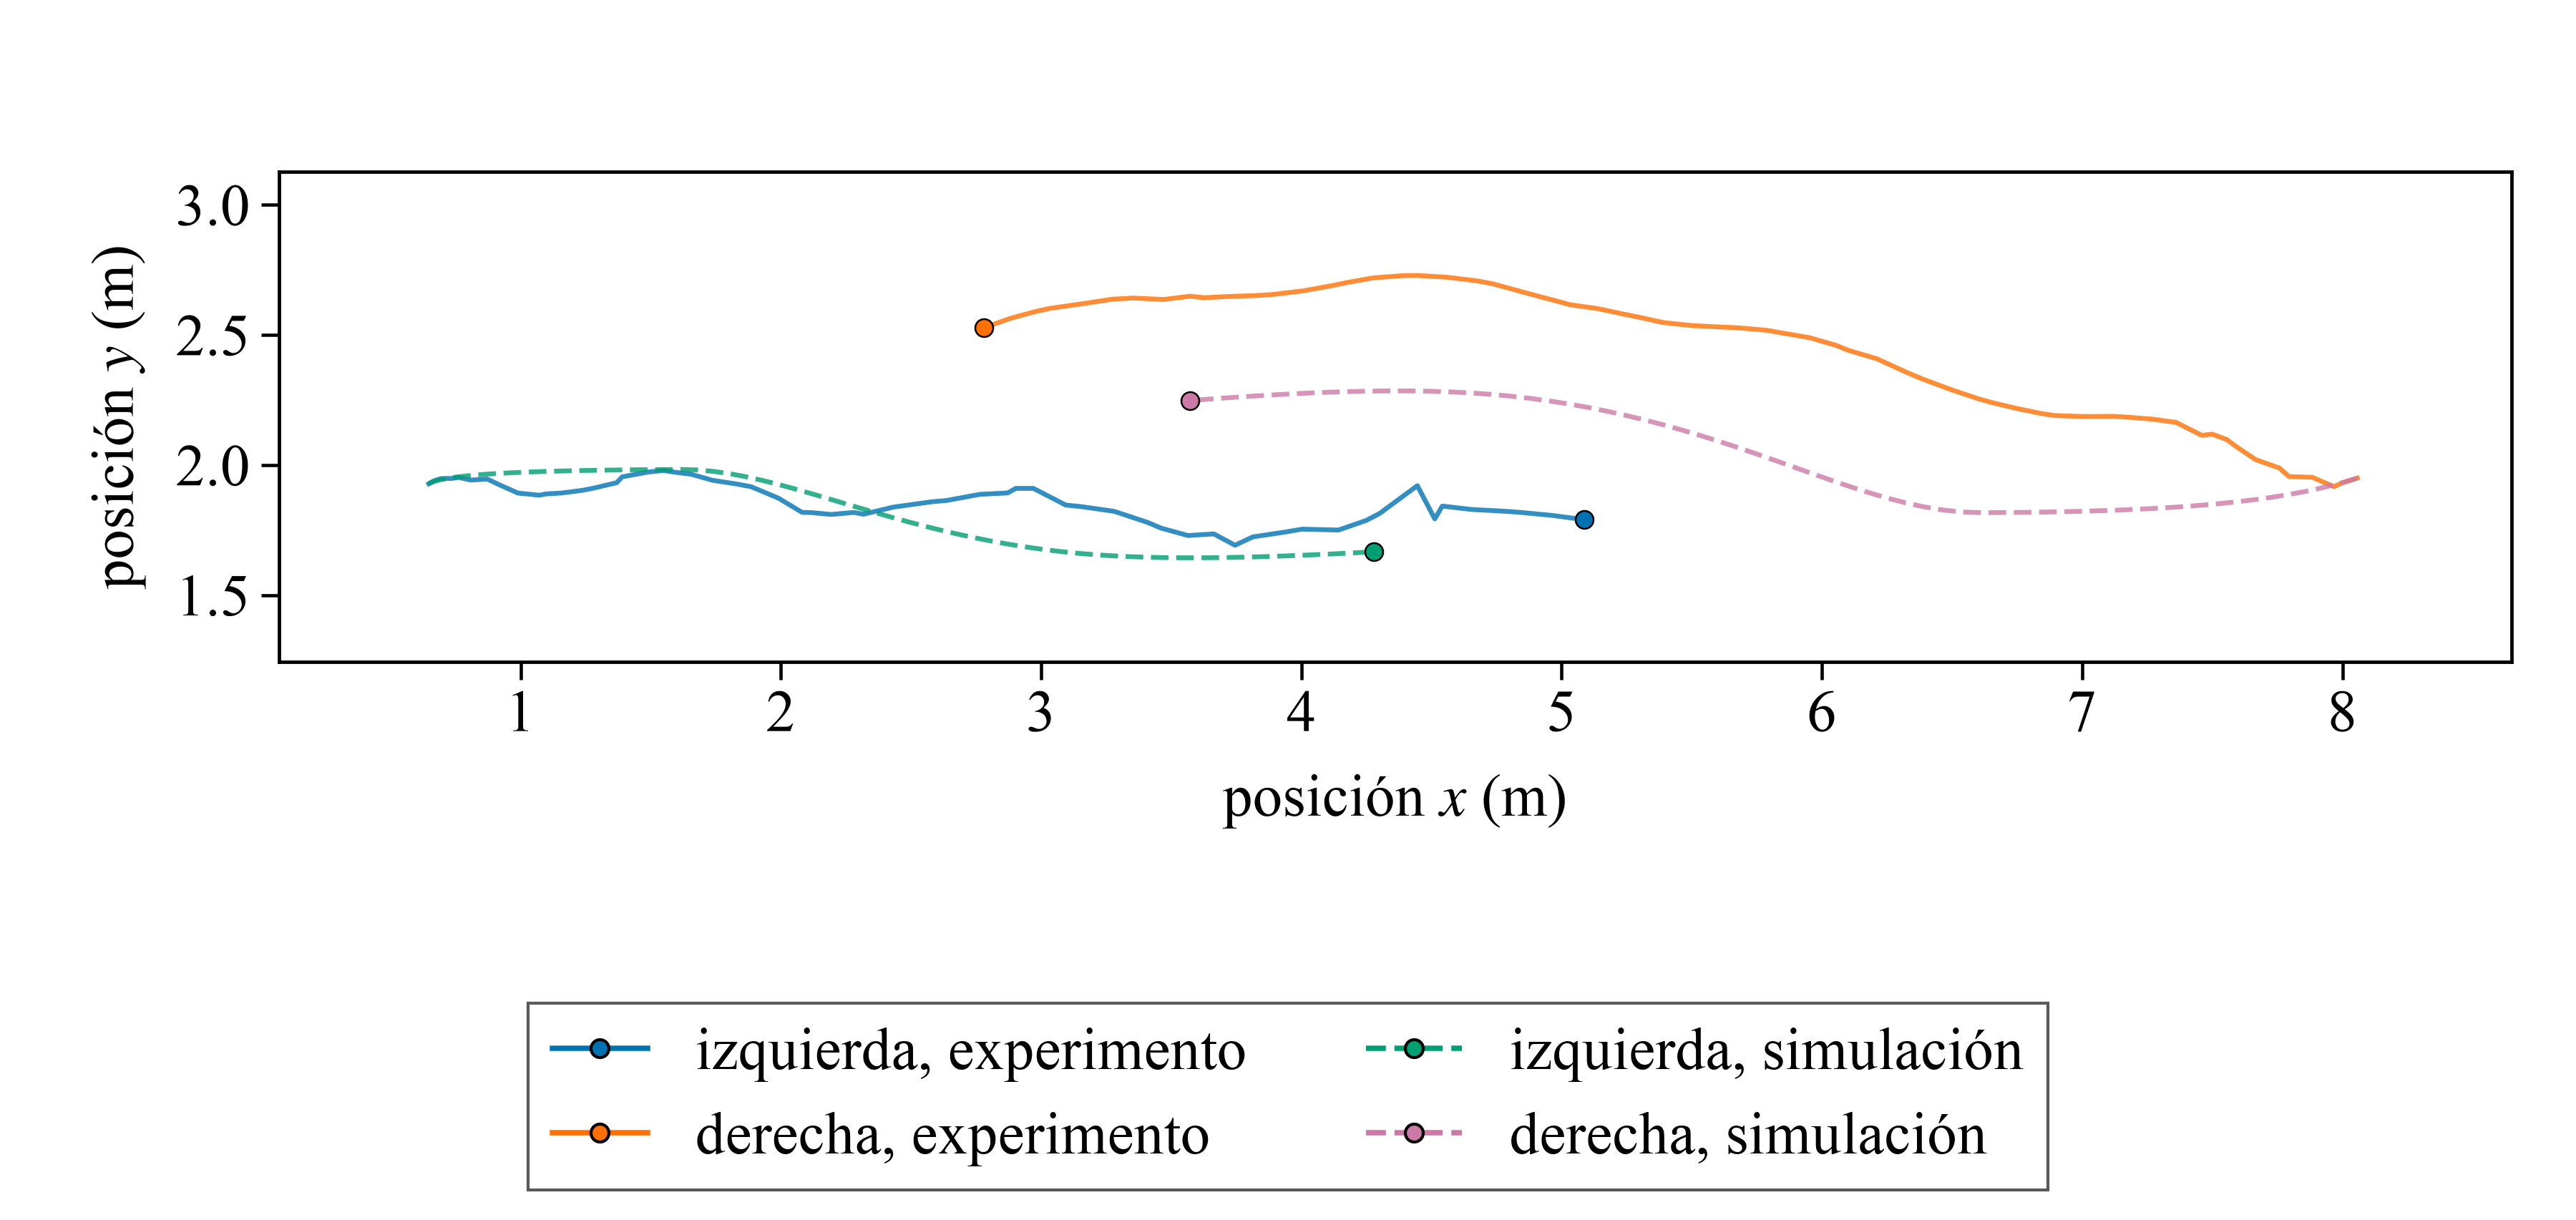
\includegraphics[width=\linewidth,height=0.52\textheight,keepaspectratio]{anim_b.png}
      \par\smallskip{\scriptsize\url{https://youtu.be/PENDIENTE}}
    \end{column}
  \end{columns}
  \vspace{6pt}
  \centering{\small $\dlat = 0.25\uni{m}$, \quad $\dact = 5\uni{m}$}
\end{frame}

\begin{frame}{Resultados}
  \framesubtitle{Trayectorias: experimento y simulación}
  \centering
  {\small Evento 15}\par
  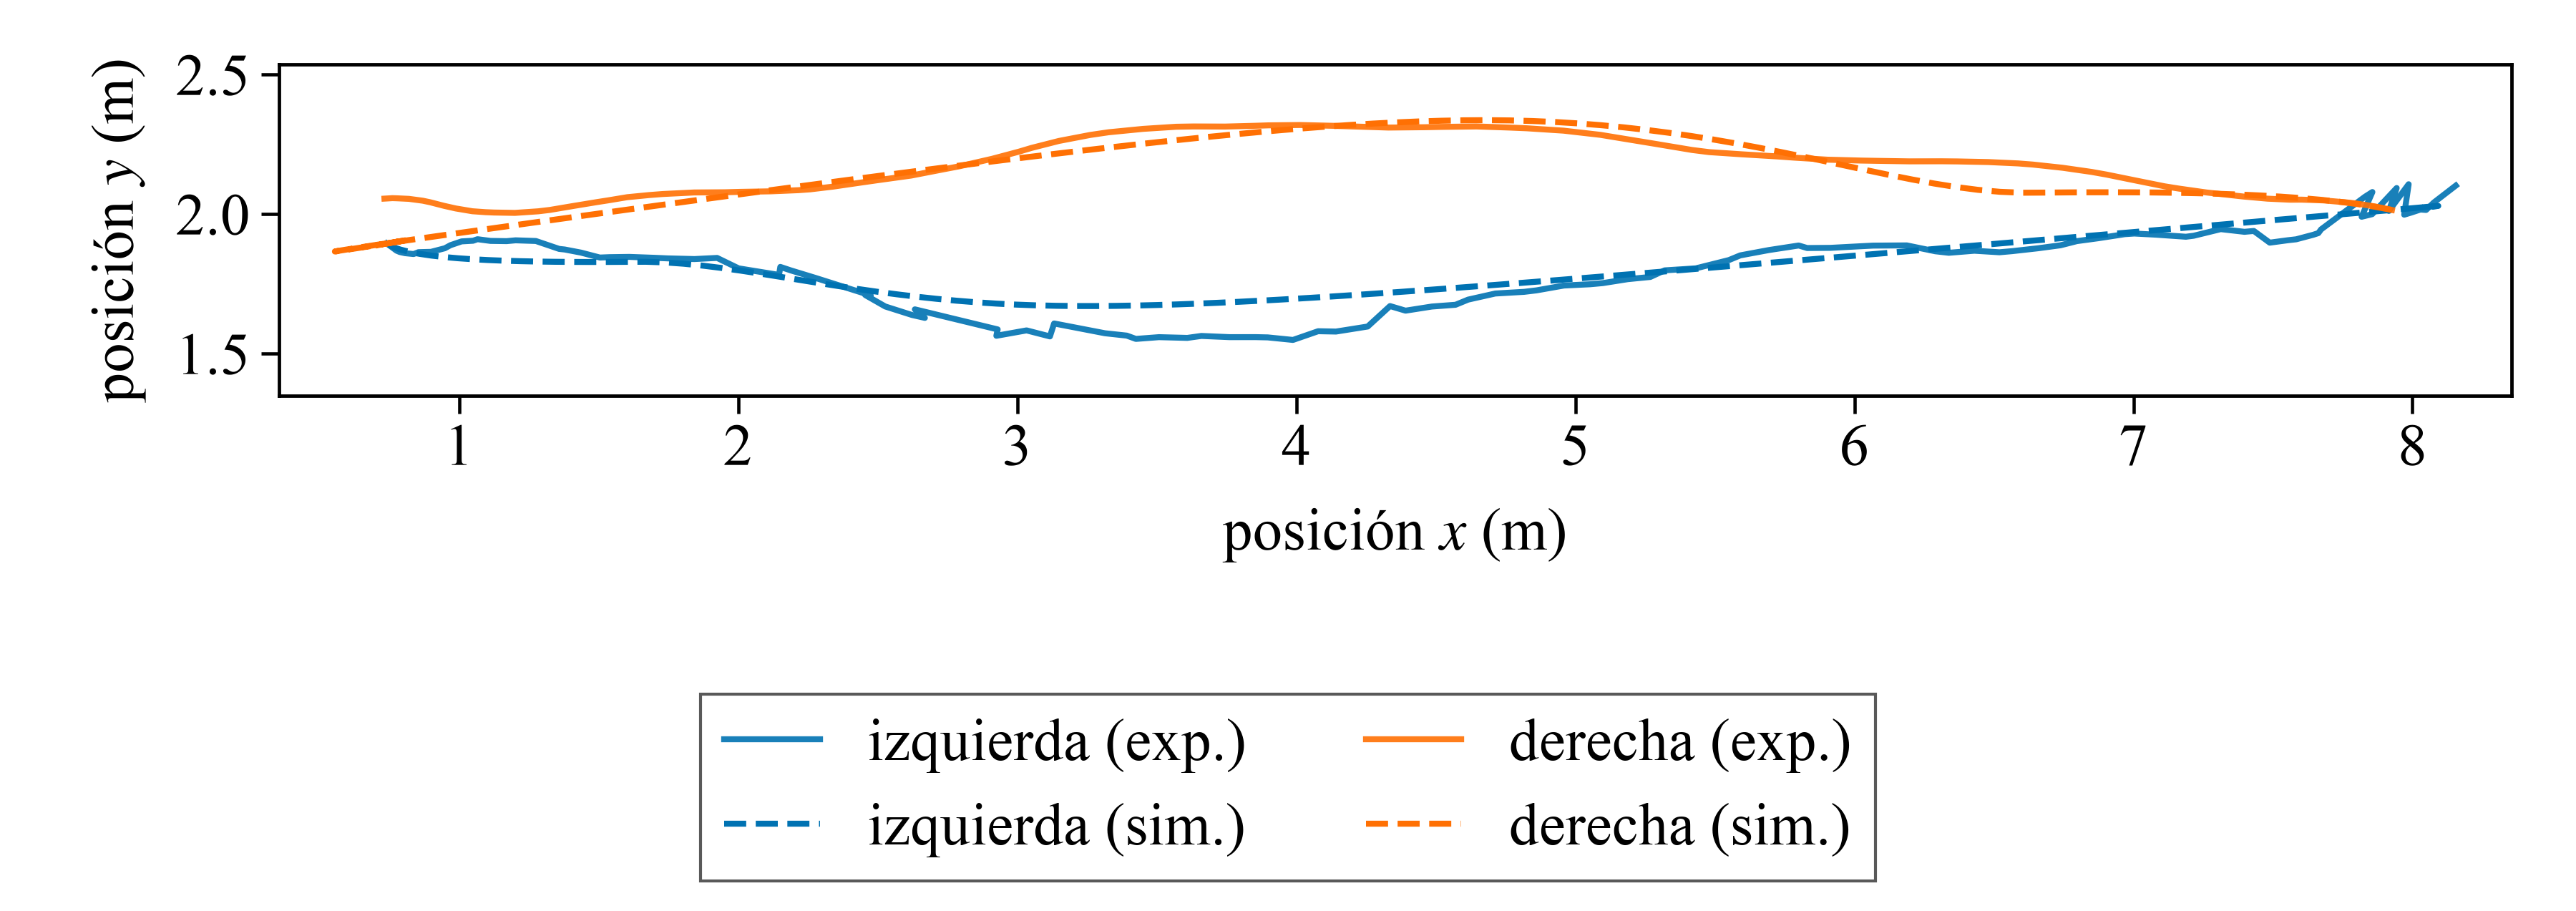
\includegraphics[width=\linewidth,height=0.36\textheight,keepaspectratio]{tray_a.png}\par
  \vspace{2pt}
  {\small Evento 11}\par
  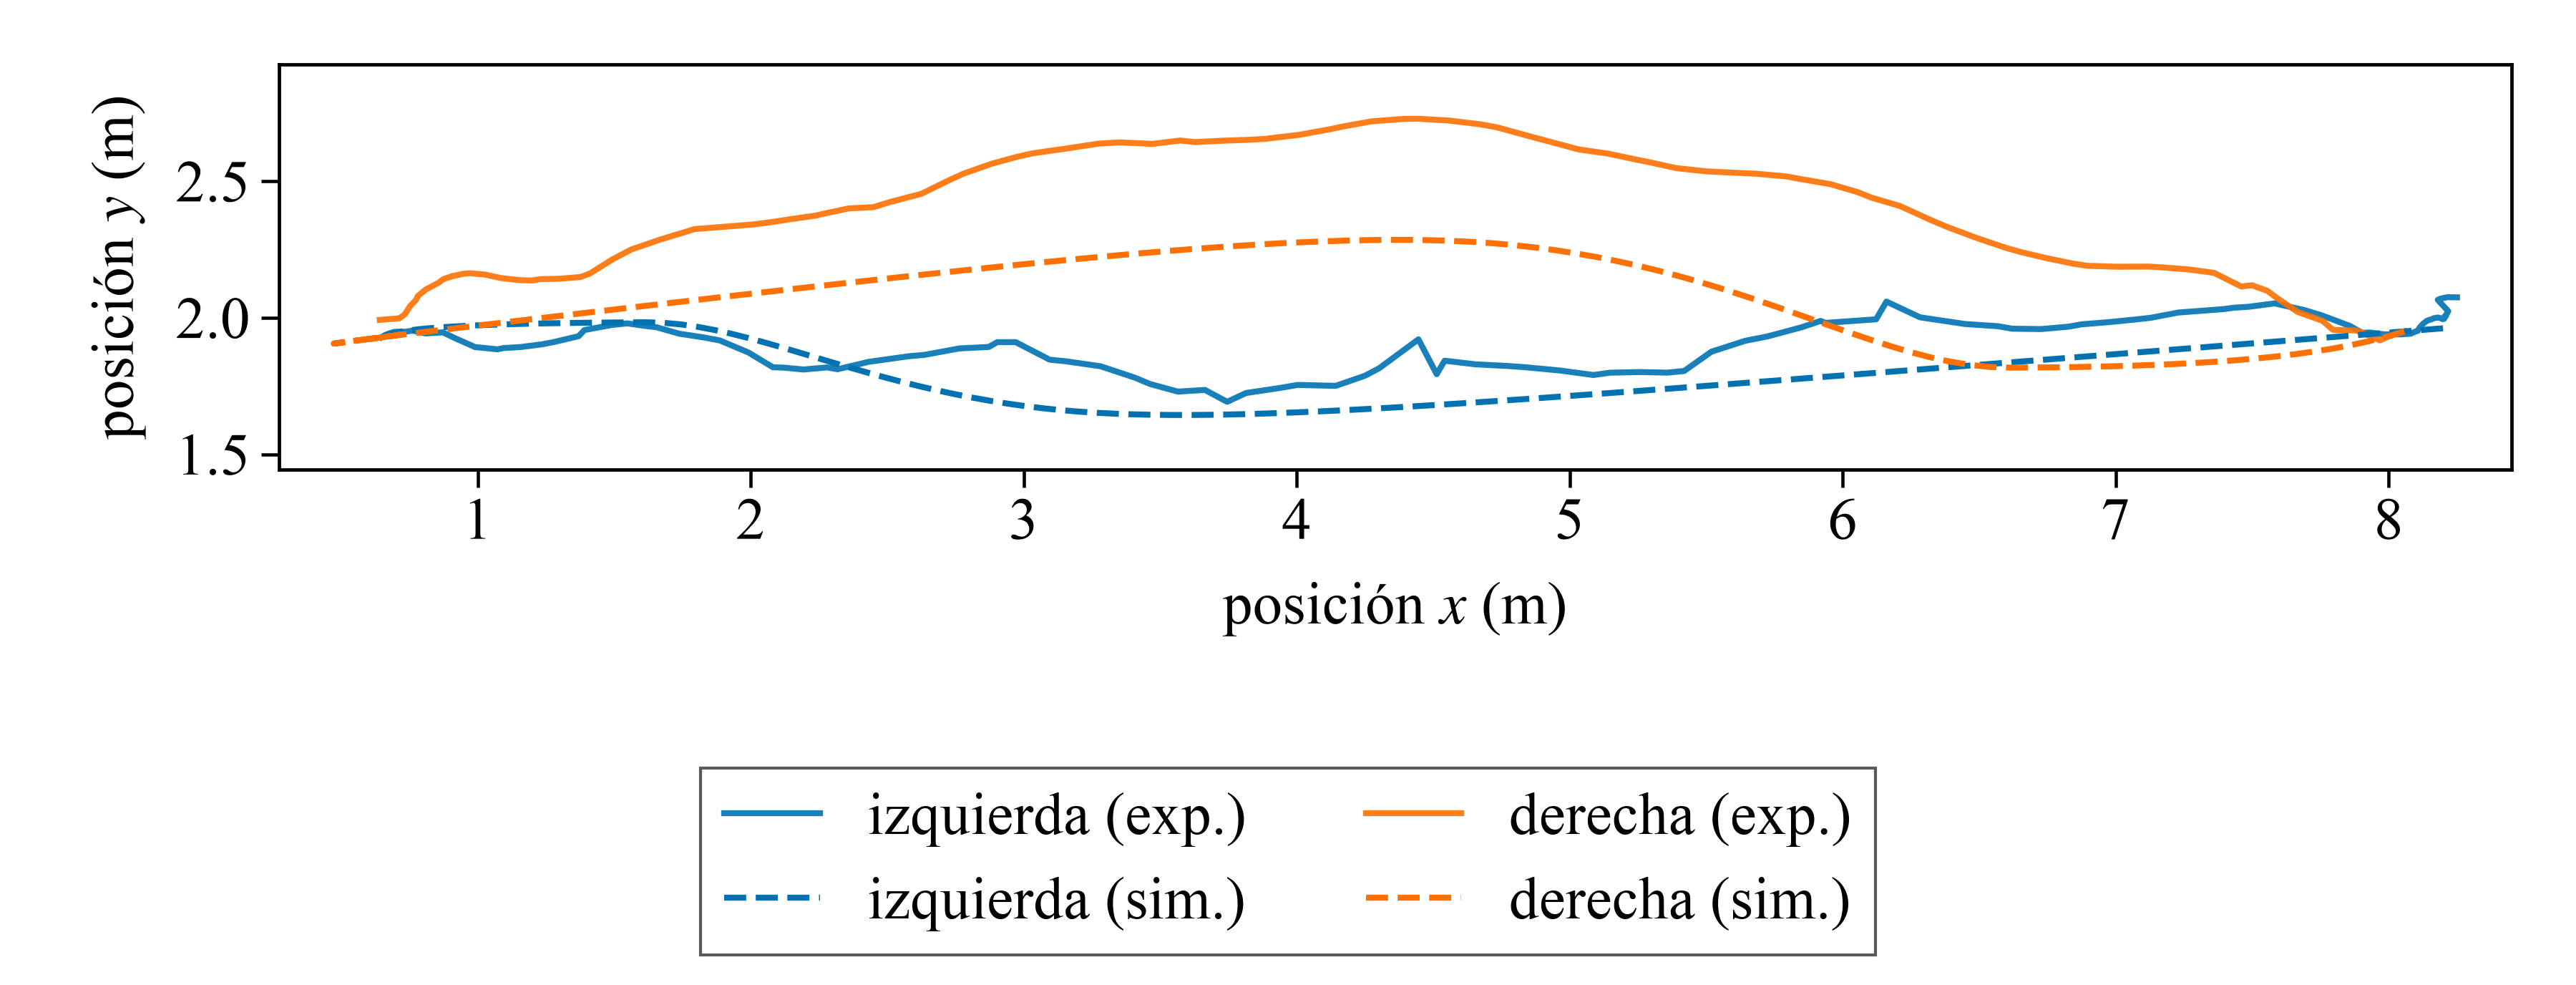
\includegraphics[width=\linewidth,height=0.36\textheight,keepaspectratio]{tray_b.png}
\end{frame}

\begin{frame}{Resultados}
  \framesubtitle{Evolución temporal del observable: métrica 1}
  \begin{columns}[T]
    \begin{column}{0.49\textwidth}
      \centering{\small Evento 15}\par\smallskip
      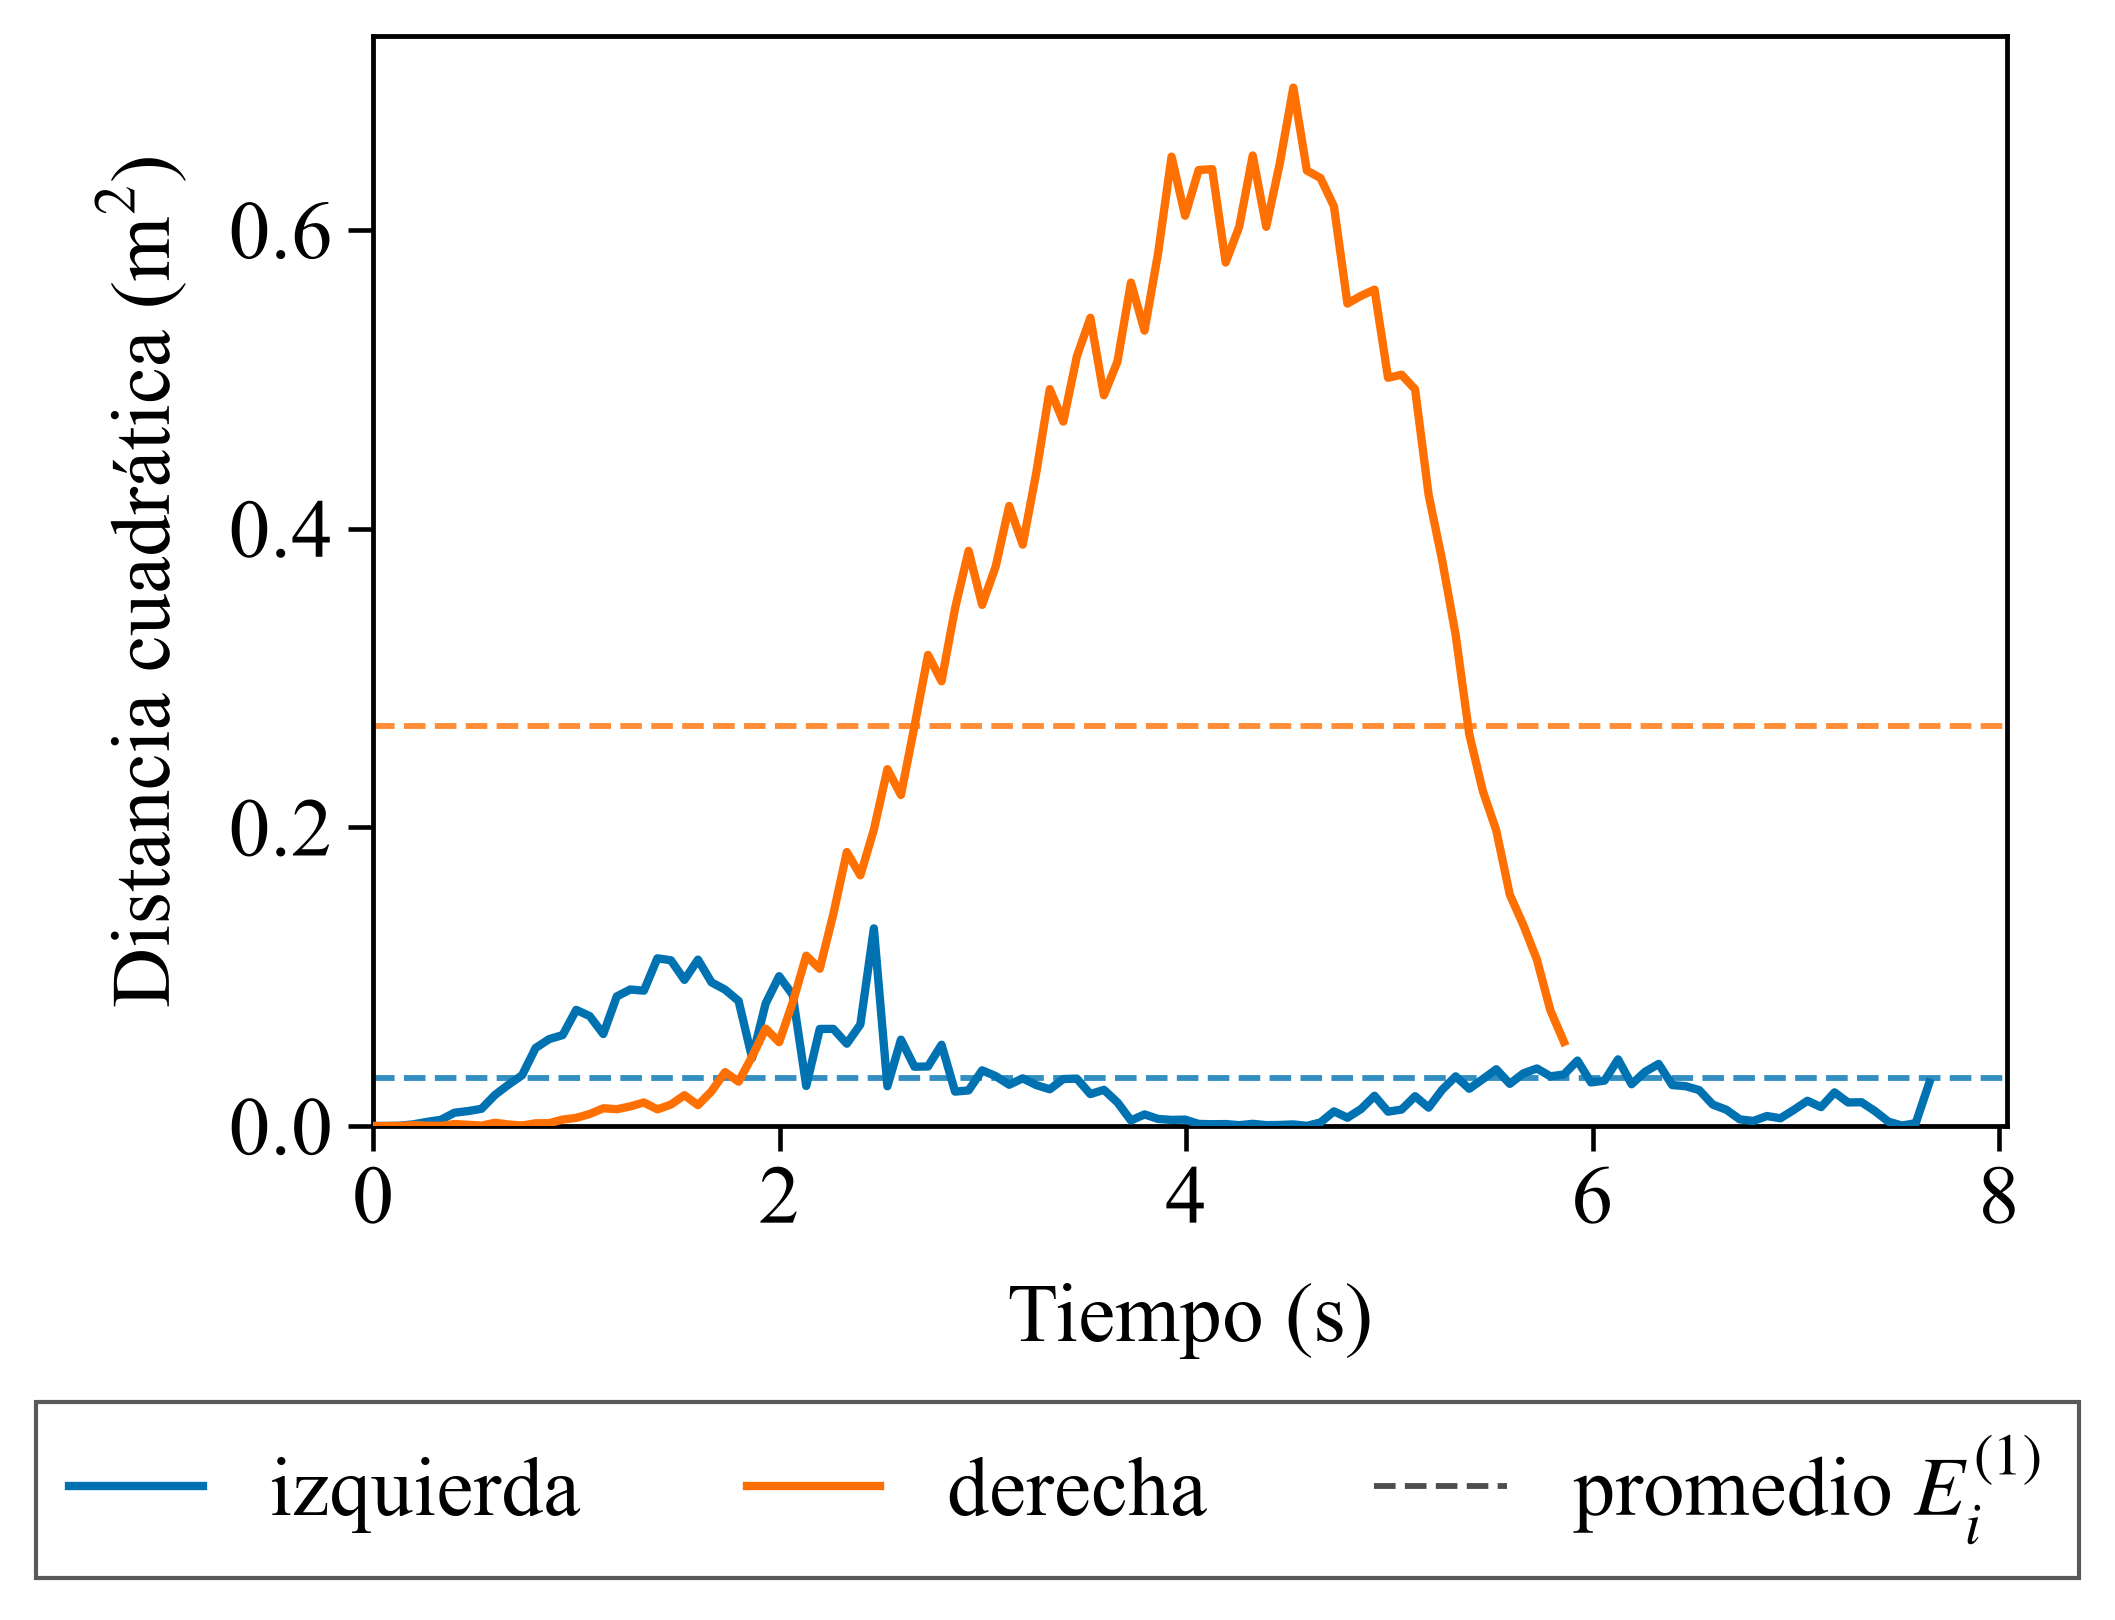
\includegraphics[width=\linewidth,height=0.60\textheight,keepaspectratio]{evol_E1_a.png}
    \end{column}
    \begin{column}{0.49\textwidth}
      \centering{\small Evento 11}\par\smallskip
      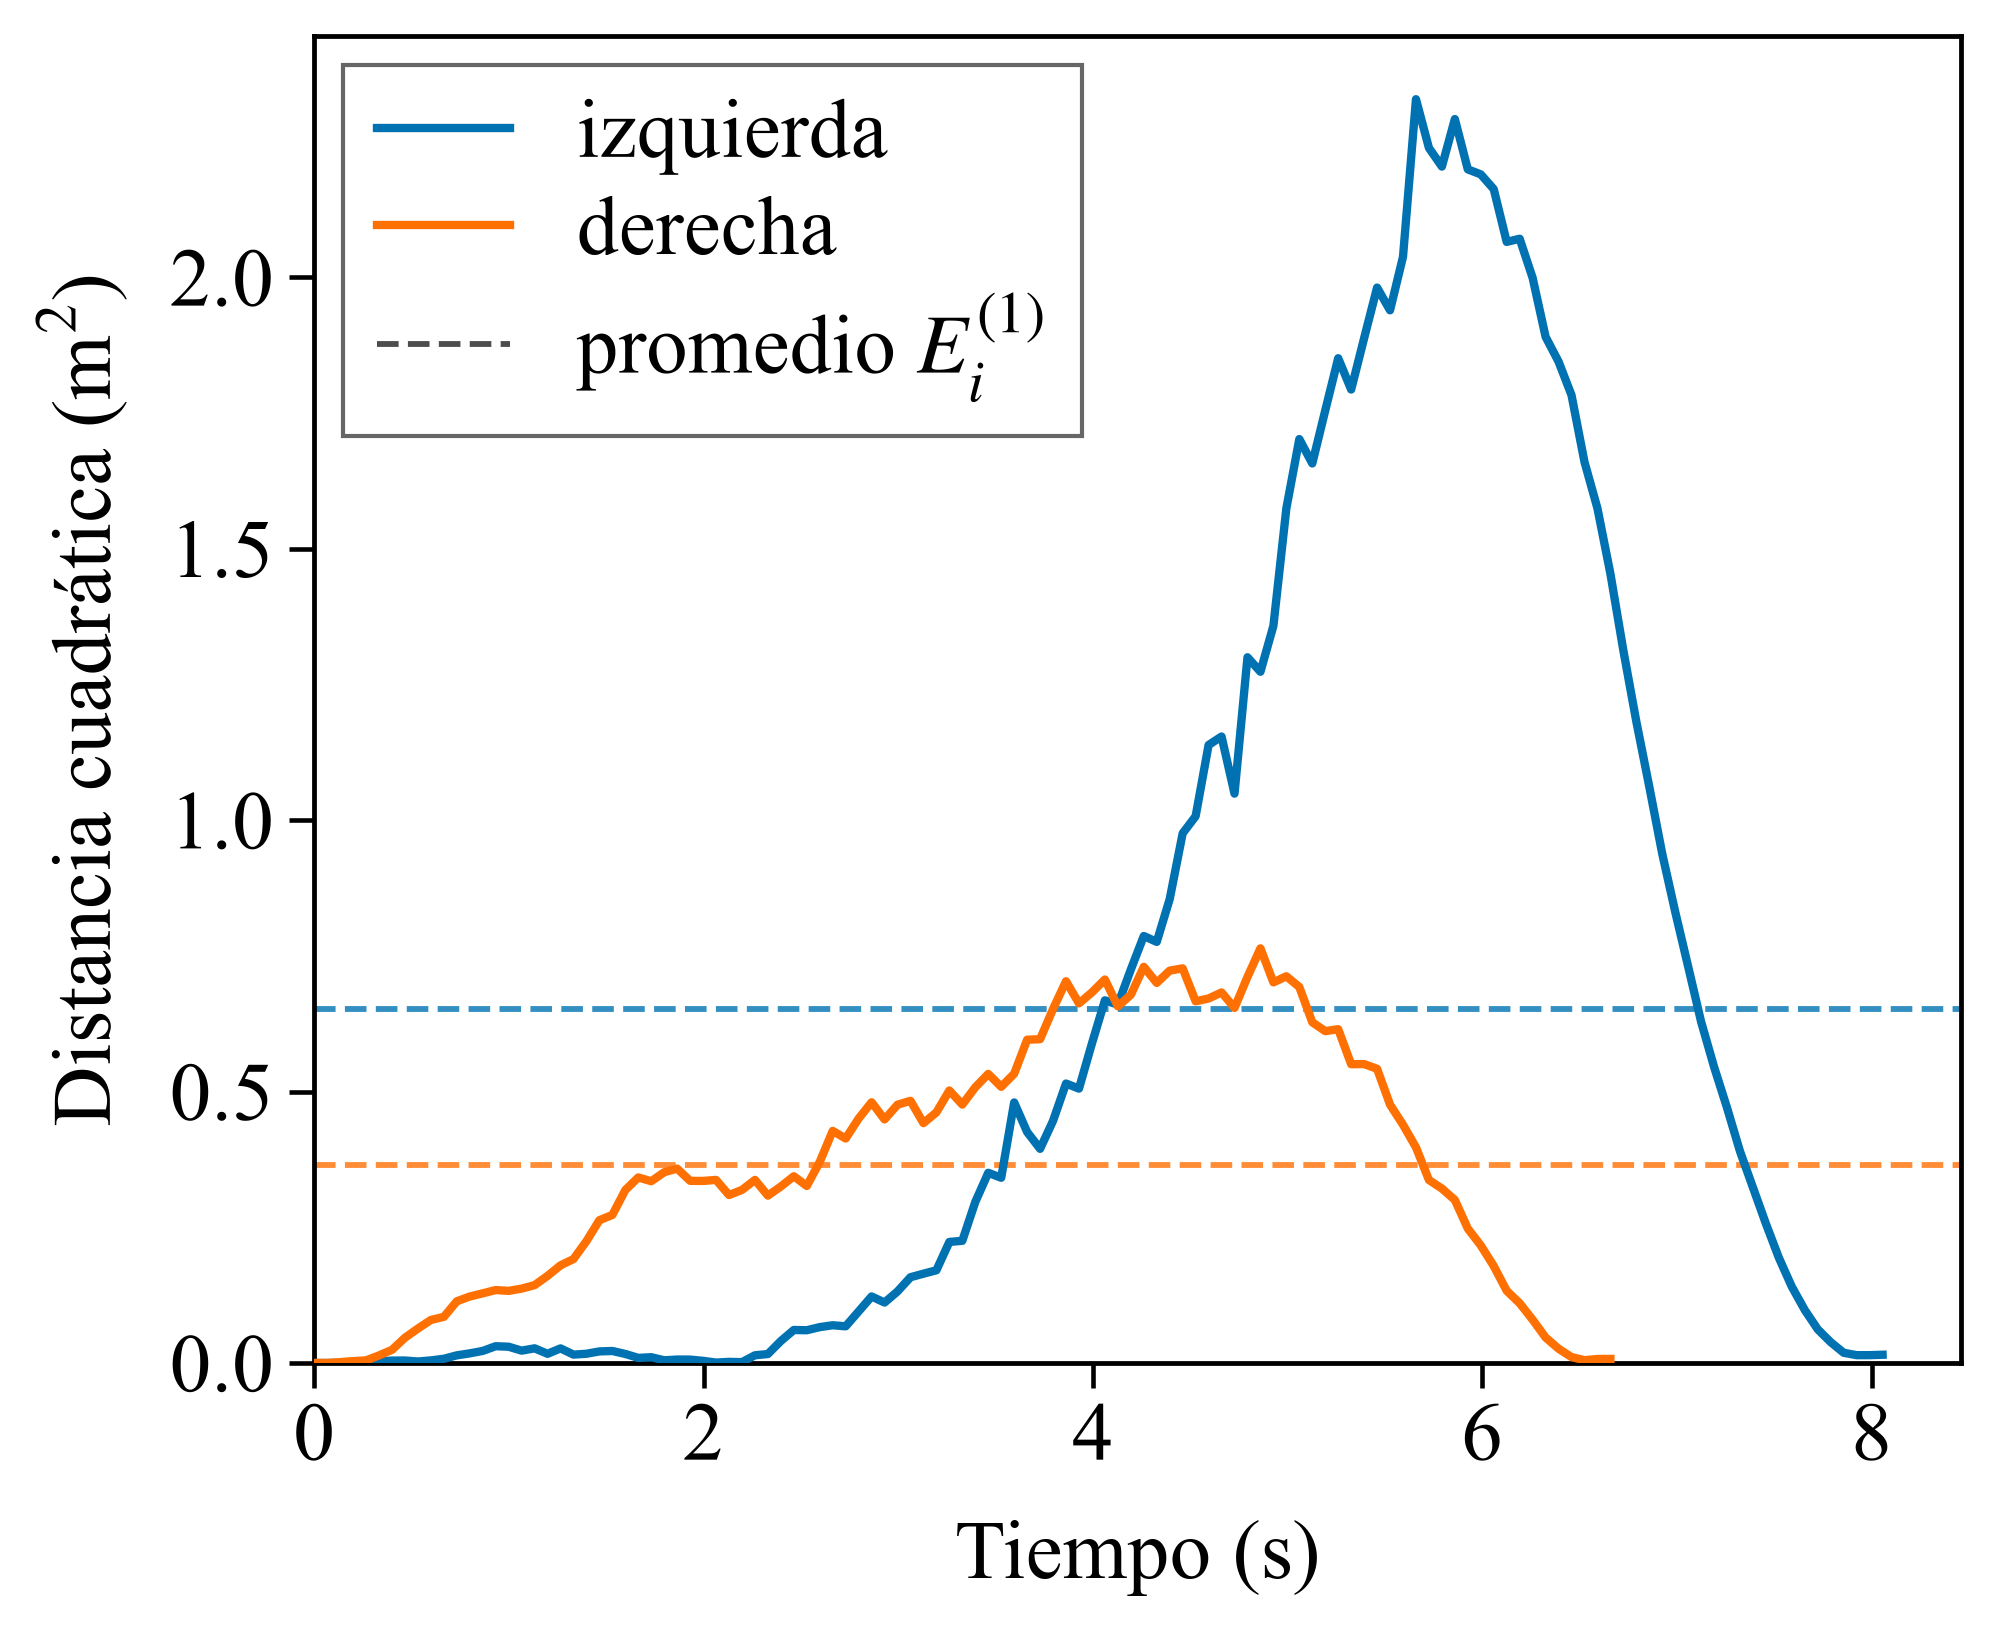
\includegraphics[width=\linewidth,height=0.60\textheight,keepaspectratio]{evol_E1_b.png}
    \end{column}
  \end{columns}
  \vspace{4pt}
  \centering{\small $d^2_i(t_k) = \big|\vv{r}^{\,exp}_i(t_k) - \vv{r}^{\,sim}_i(t_k)\big|^2$, \quad
    punteada: $E^{(1)}_i = \frac{1}{N_m}\sum_k d^2_i(t_k)$, \quad
    $\dlat = 0.25\uni{m}$, \ $\dact = 5\uni{m}$}
\end{frame}

\begin{frame}{Resultados}
  \framesubtitle{Evolución temporal del observable: métrica 2}
  \begin{columns}[T]
    \begin{column}{0.49\textwidth}
      \centering{\small Evento 15}\par\smallskip
      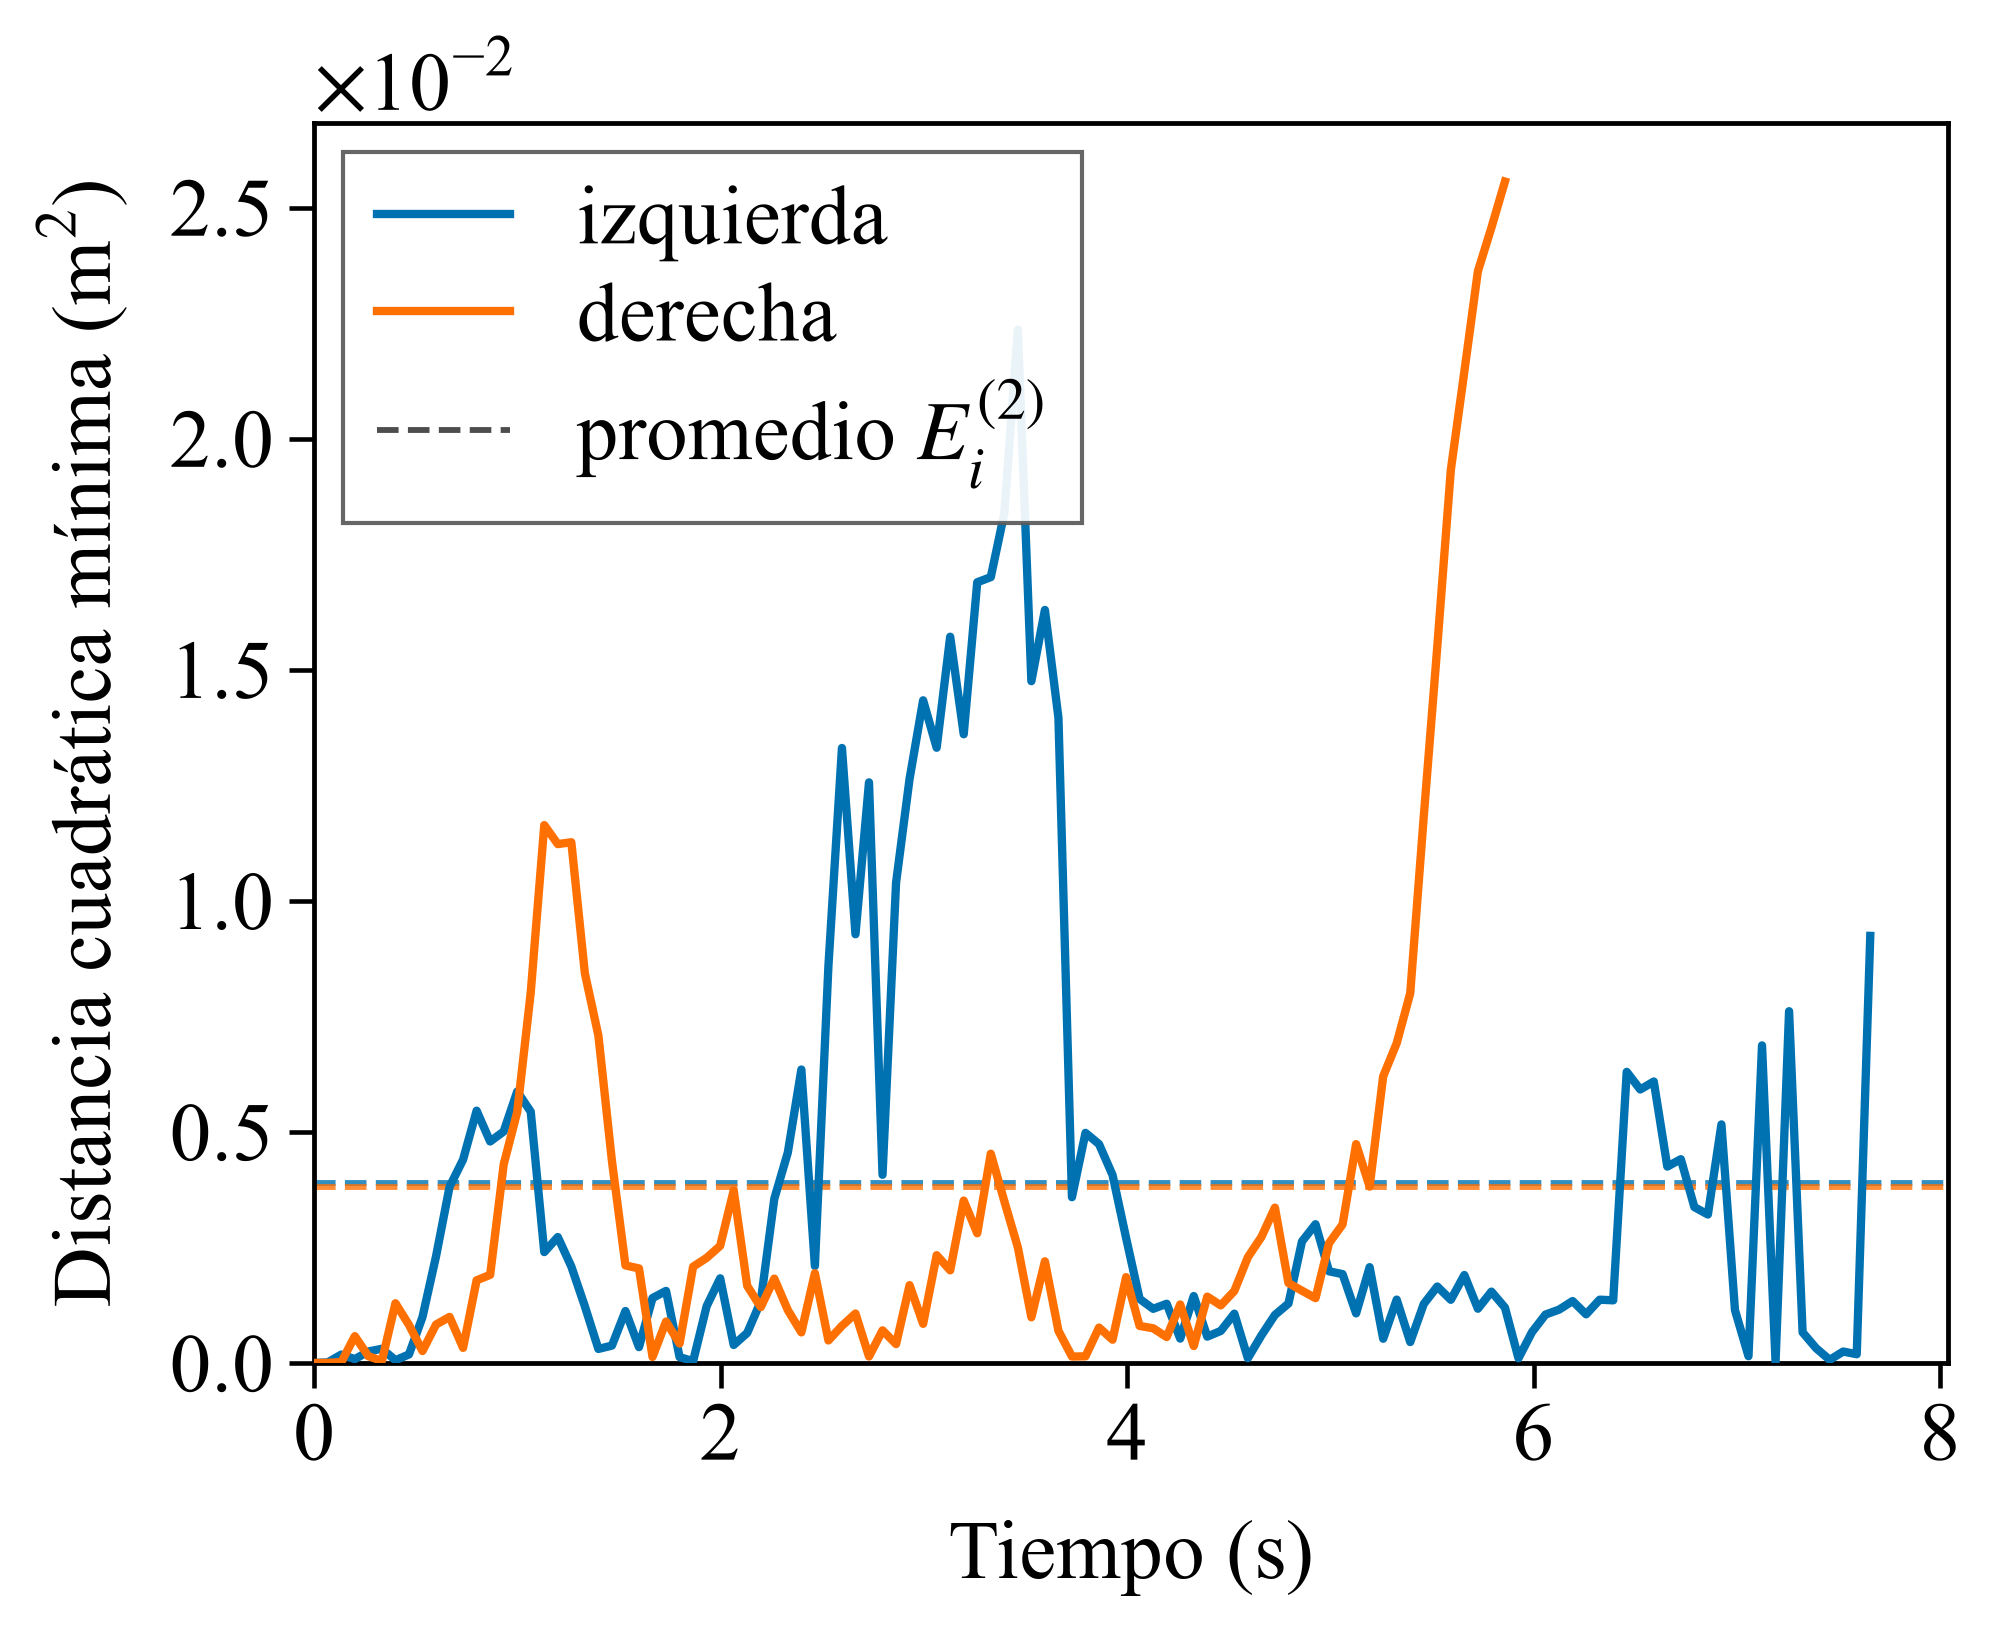
\includegraphics[width=\linewidth,height=0.60\textheight,keepaspectratio]{evol_E2_a.png}
    \end{column}
    \begin{column}{0.49\textwidth}
      \centering{\small Evento 11}\par\smallskip
      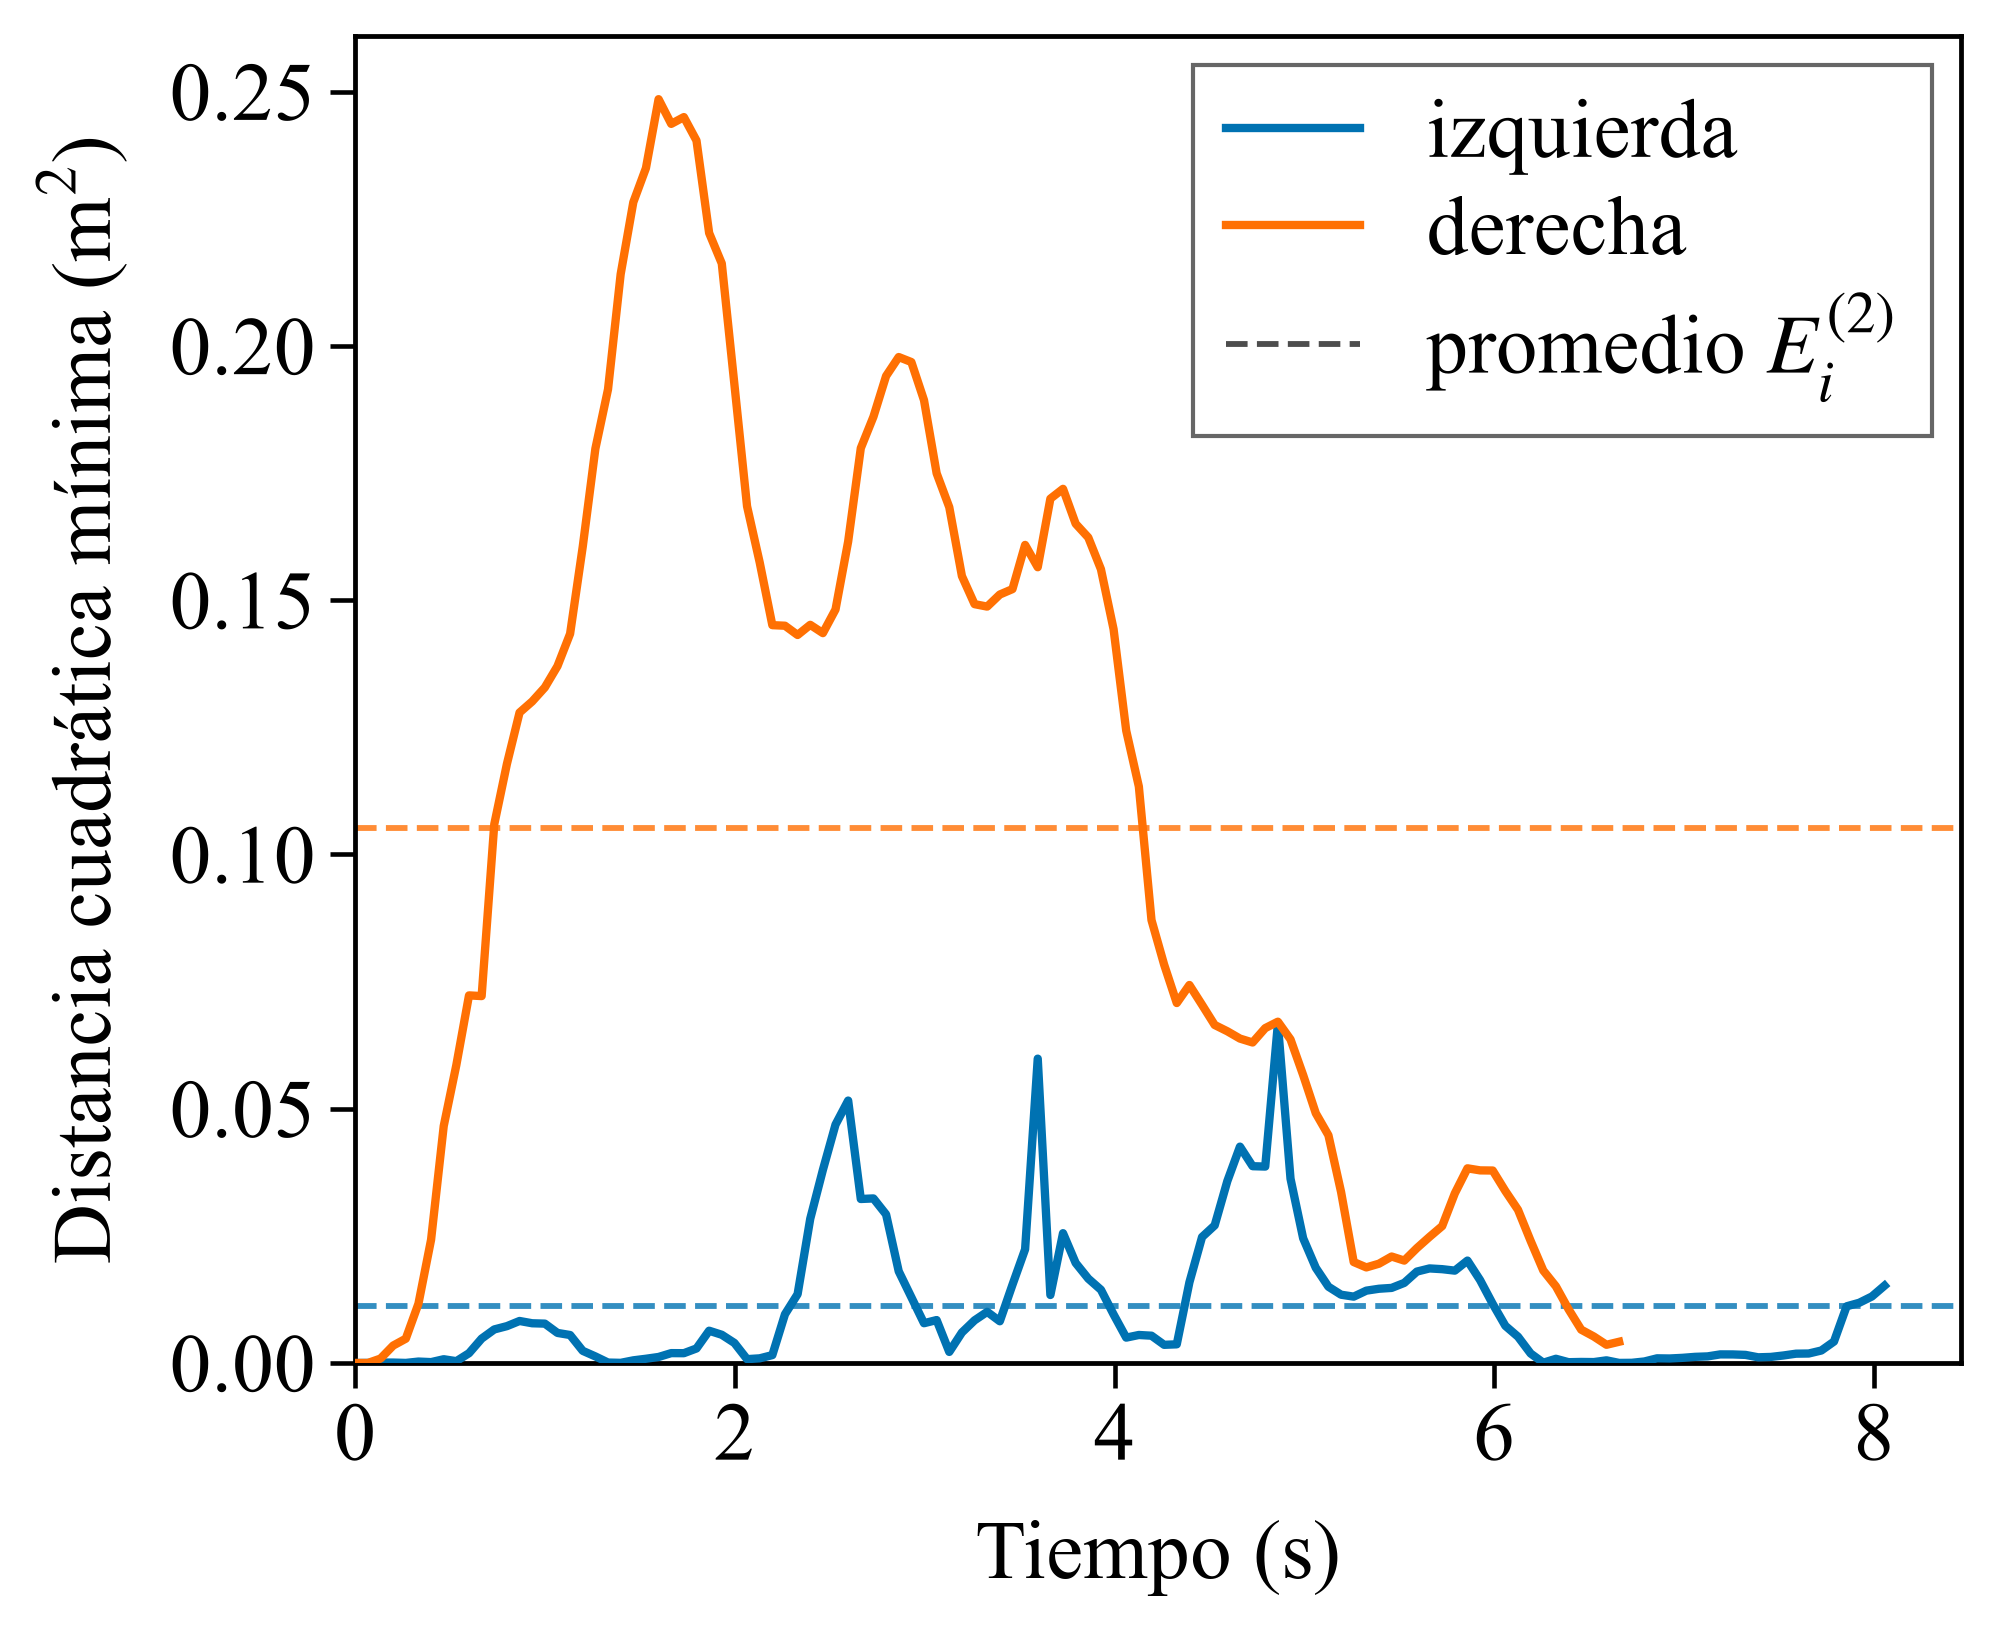
\includegraphics[width=\linewidth,height=0.60\textheight,keepaspectratio]{evol_E2_b.png}
    \end{column}
  \end{columns}
  \vspace{4pt}
  \centering{\small $d^2_{i,\min}(t_k) = \min_j\big|\vv{r}^{\,exp}_i(t_k) - \vv{r}^{\,sim}_i(t_j)\big|^2$, \quad
    punteada: $E^{(2)}_i = \frac{1}{N_m}\sum_k d^2_{i,\min}(t_k)$, \quad
    $\dlat = 0.25\uni{m}$, \ $\dact = 5\uni{m}$}
\end{frame}

\begin{frame}{Resultados}
  \framesubtitle{Calibración poblacional: métrica 1}
  \begin{cols}
    \begin{column}{0.62\textwidth}
      \figura{E1_superficie.png}
    \end{column}
    \begin{column}{0.34\textwidth}
      \begin{resultado}[Óptimo]
        \item $\dlat = 0.20\uni{m}$
        \item $\dact = 4\uni{m}$
        \item $\langle E^{(1)}\rangle = 0.4 \pm 0.3\uni{m^2}$
      \end{resultado}
    \end{column}
  \end{cols}
\end{frame}

\begin{frame}{Resultados}
  \framesubtitle{Calibración poblacional: métrica 1, cortes por el óptimo}
  \begin{columns}[T]
    \begin{column}{0.49\textwidth}
      \centering
      {\small Variando $\dlat$, con $\dact = 4\uni{m}$ fijo\par}
      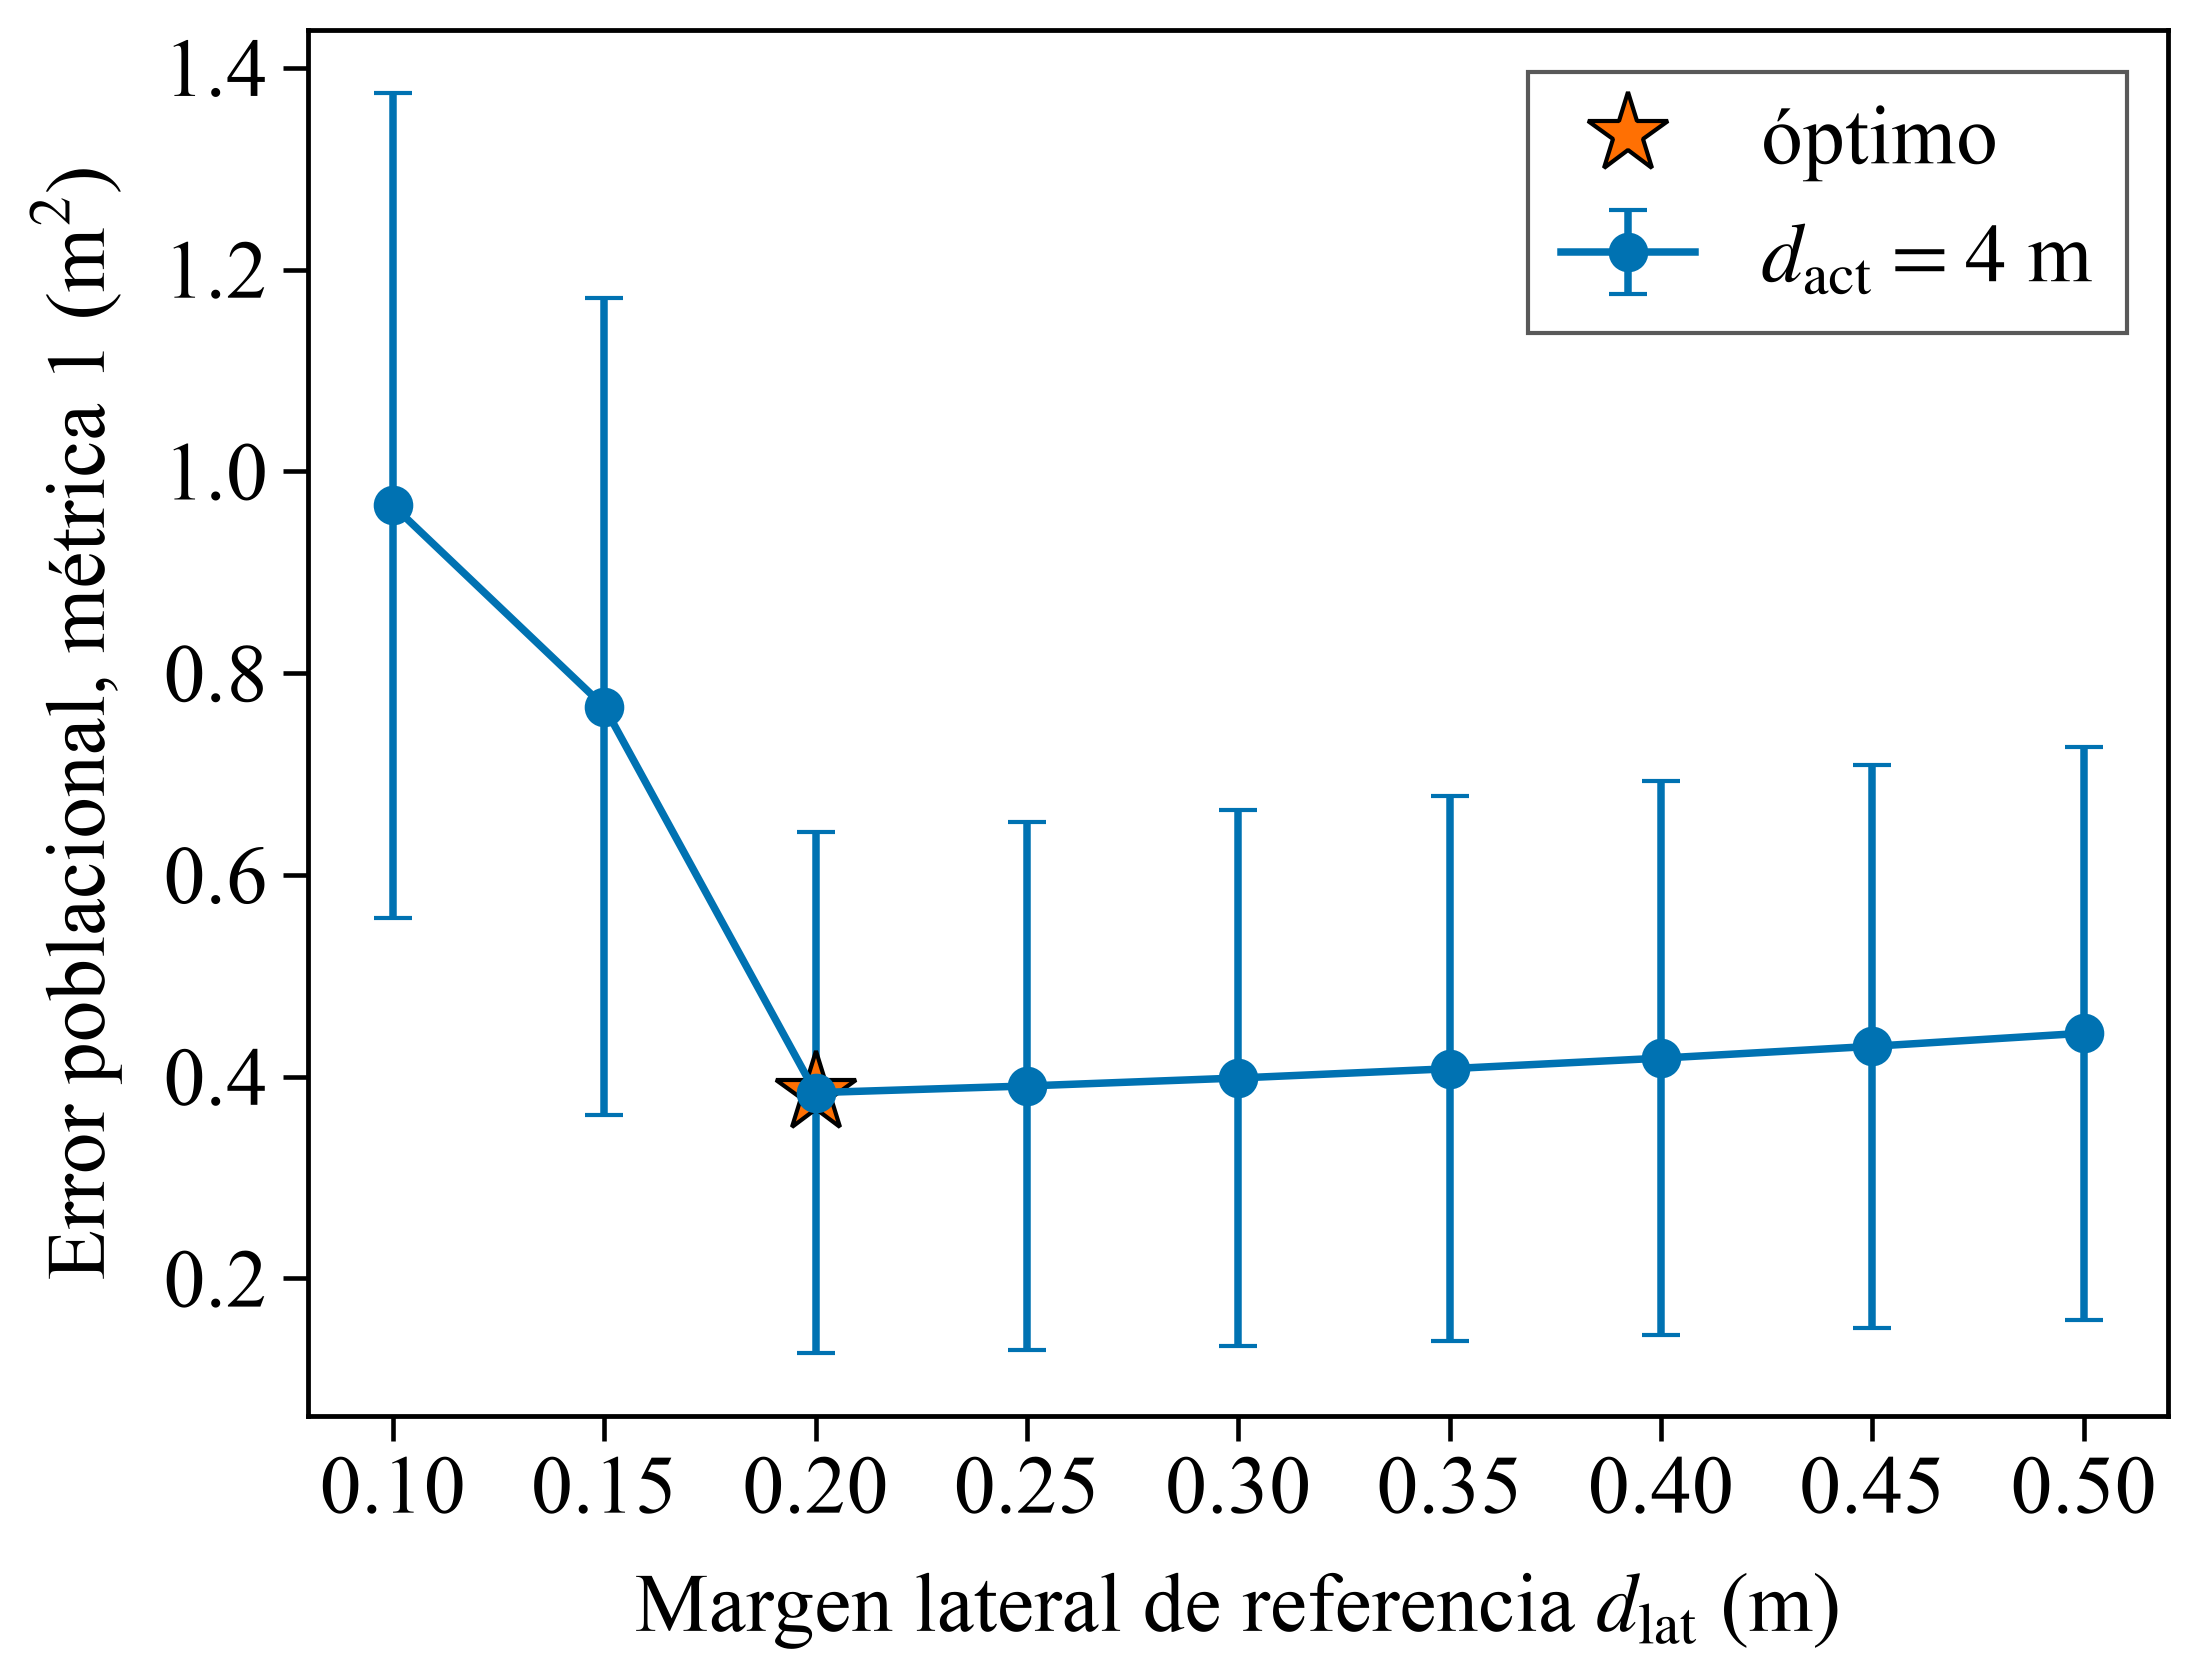
\includegraphics[width=\linewidth,height=0.62\textheight,keepaspectratio]{E1_corte_rmin.png}
    \end{column}
    \begin{column}{0.49\textwidth}
      \centering
      {\small Variando $\dact$, con $\dlat = 0.20\uni{m}$ fijo\par}
      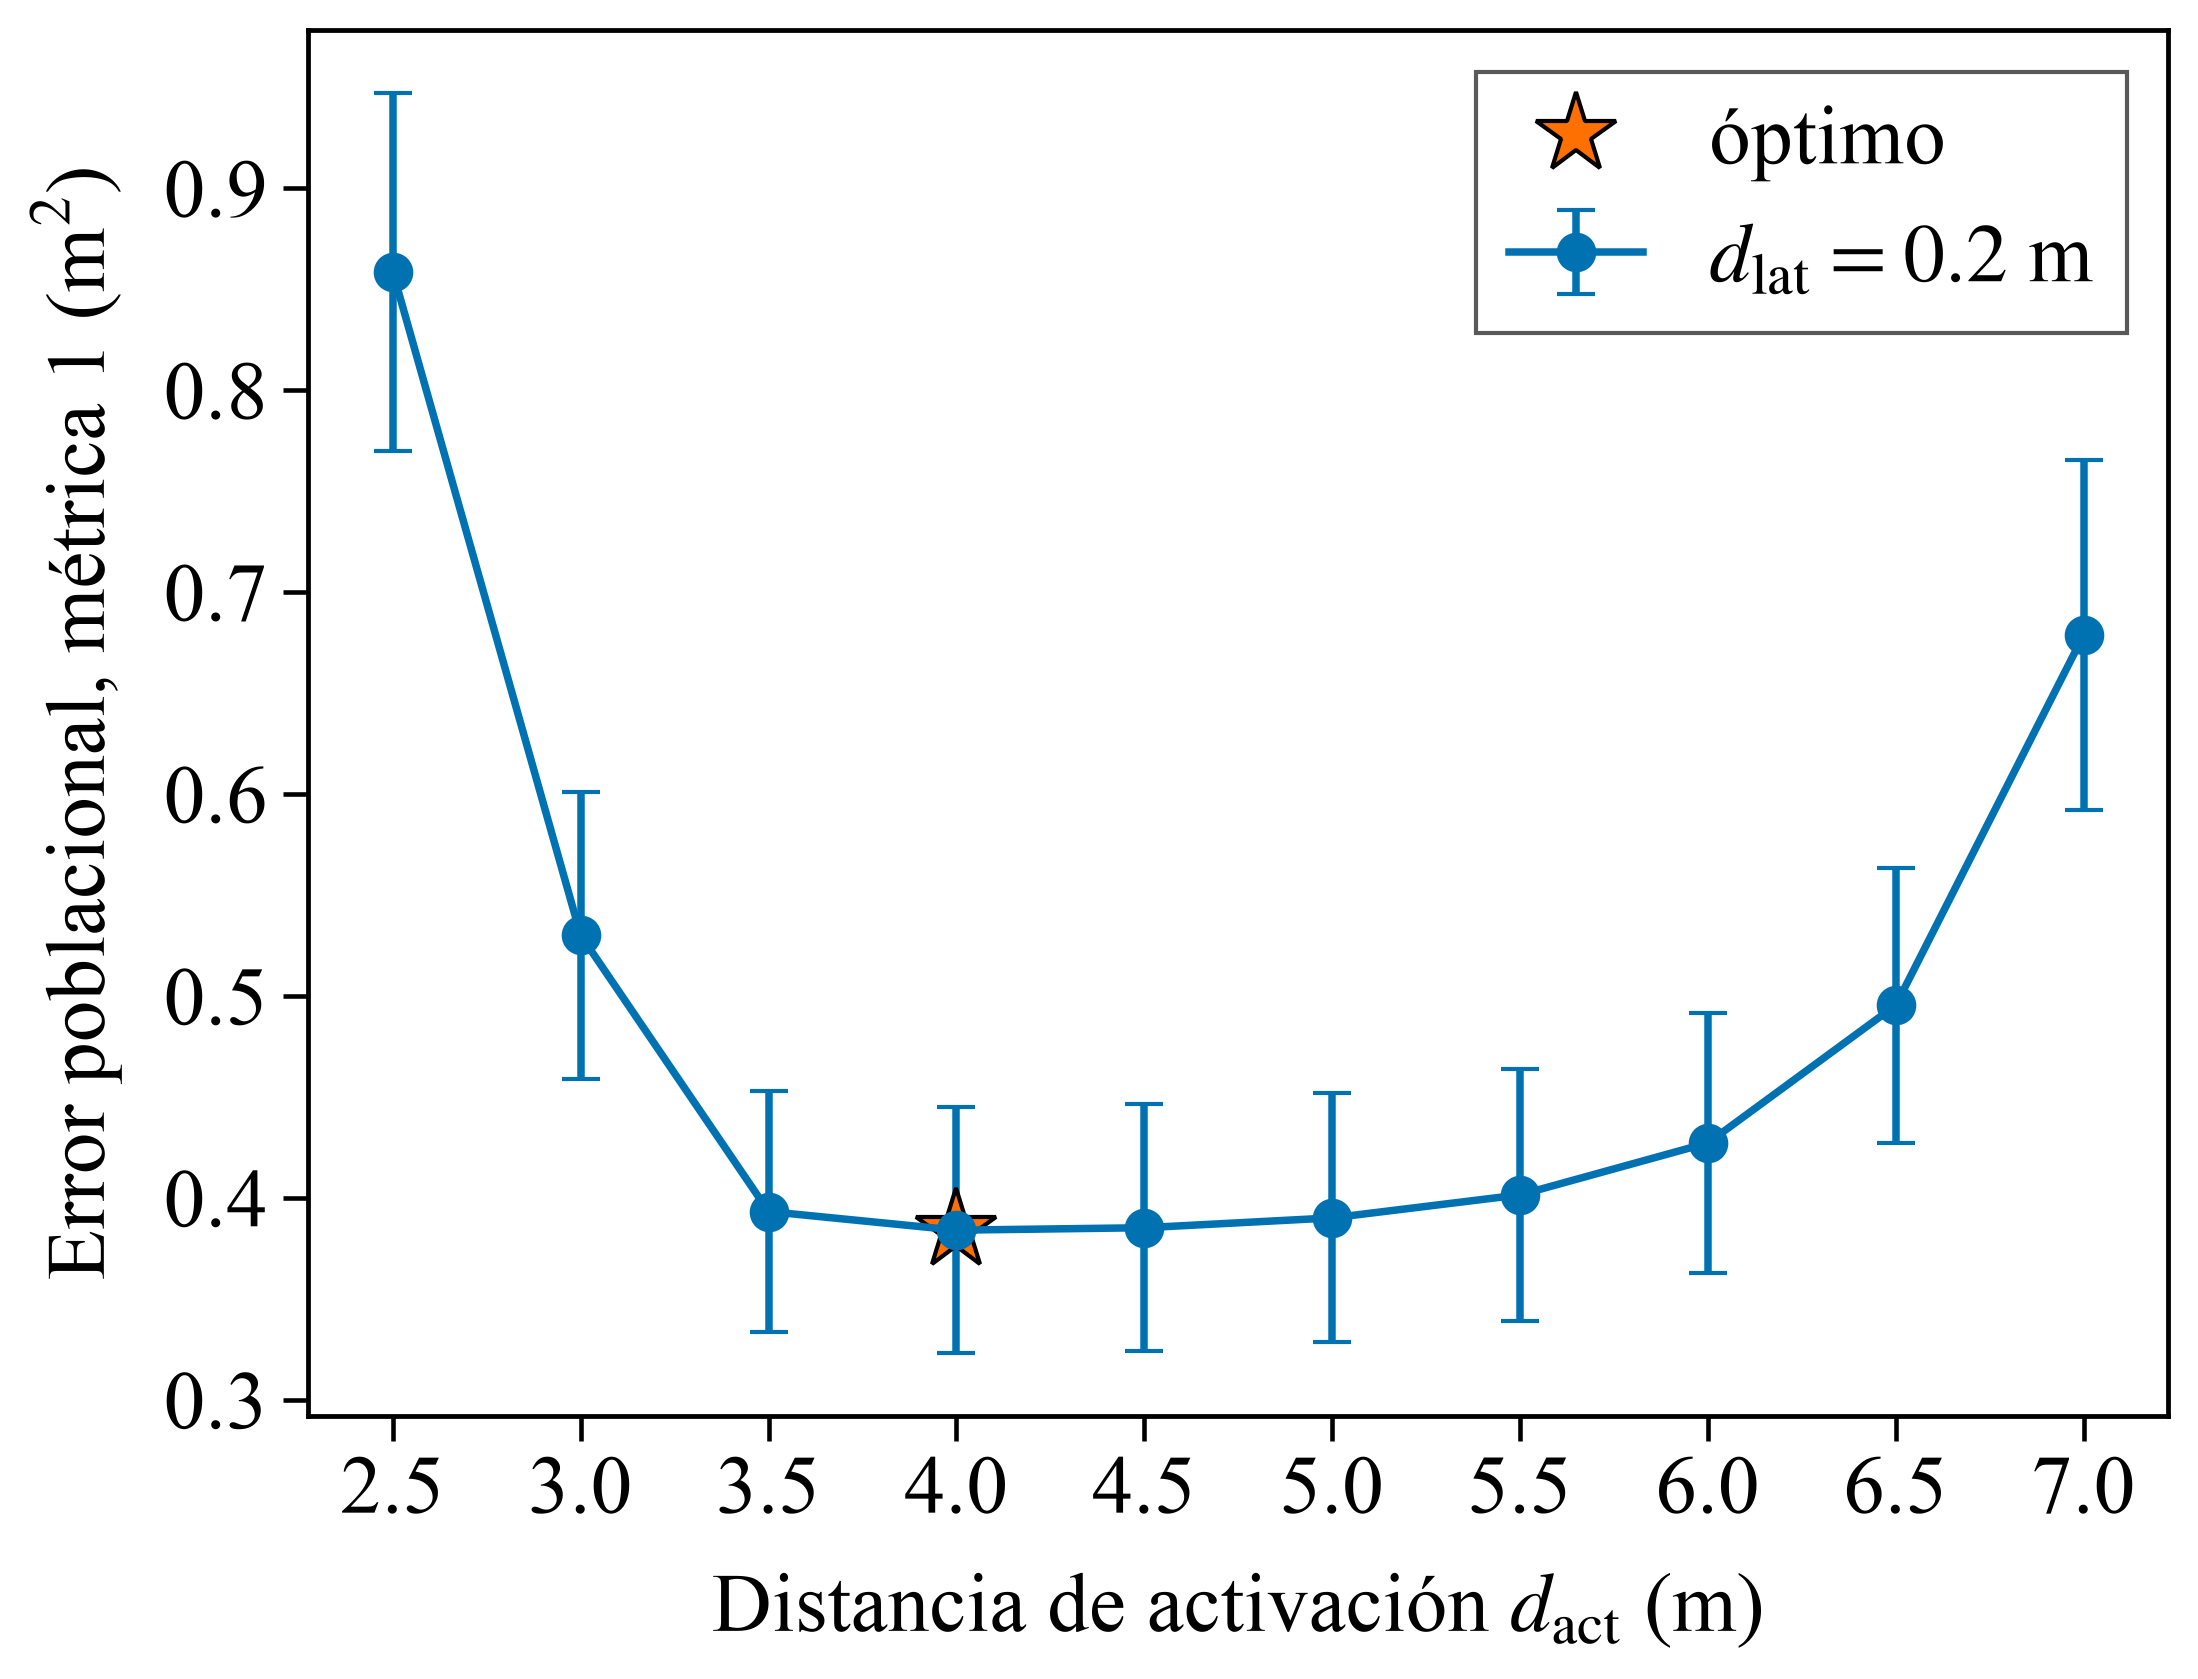
\includegraphics[width=\linewidth,height=0.62\textheight,keepaspectratio]{E1_corte_action_distance.png}
    \end{column}
  \end{columns}
\end{frame}

\begin{frame}{Resultados}
  \framesubtitle{Calibración poblacional: métrica 2}
  \begin{cols}
    \begin{column}{0.62\textwidth}
      \figura{E2_superficie.png}
    \end{column}
    \begin{column}{0.34\textwidth}
      \begin{resultado}[Óptimo]
        \item $\dlat = 0.25\uni{m}$
        \item $\dact = 5\uni{m}$
        \item $\langle E^{(2)}\rangle = (2 \pm 1)\ten{-2}\uni{m^2}$
      \end{resultado}
    \end{column}
  \end{cols}
\end{frame}

\begin{frame}{Resultados}
  \framesubtitle{Calibración poblacional: métrica 2, cortes por el óptimo}
  \begin{columns}[T]
    \begin{column}{0.49\textwidth}
      \centering
      {\small Variando $\dlat$, con $\dact = 5\uni{m}$ fijo\par}
      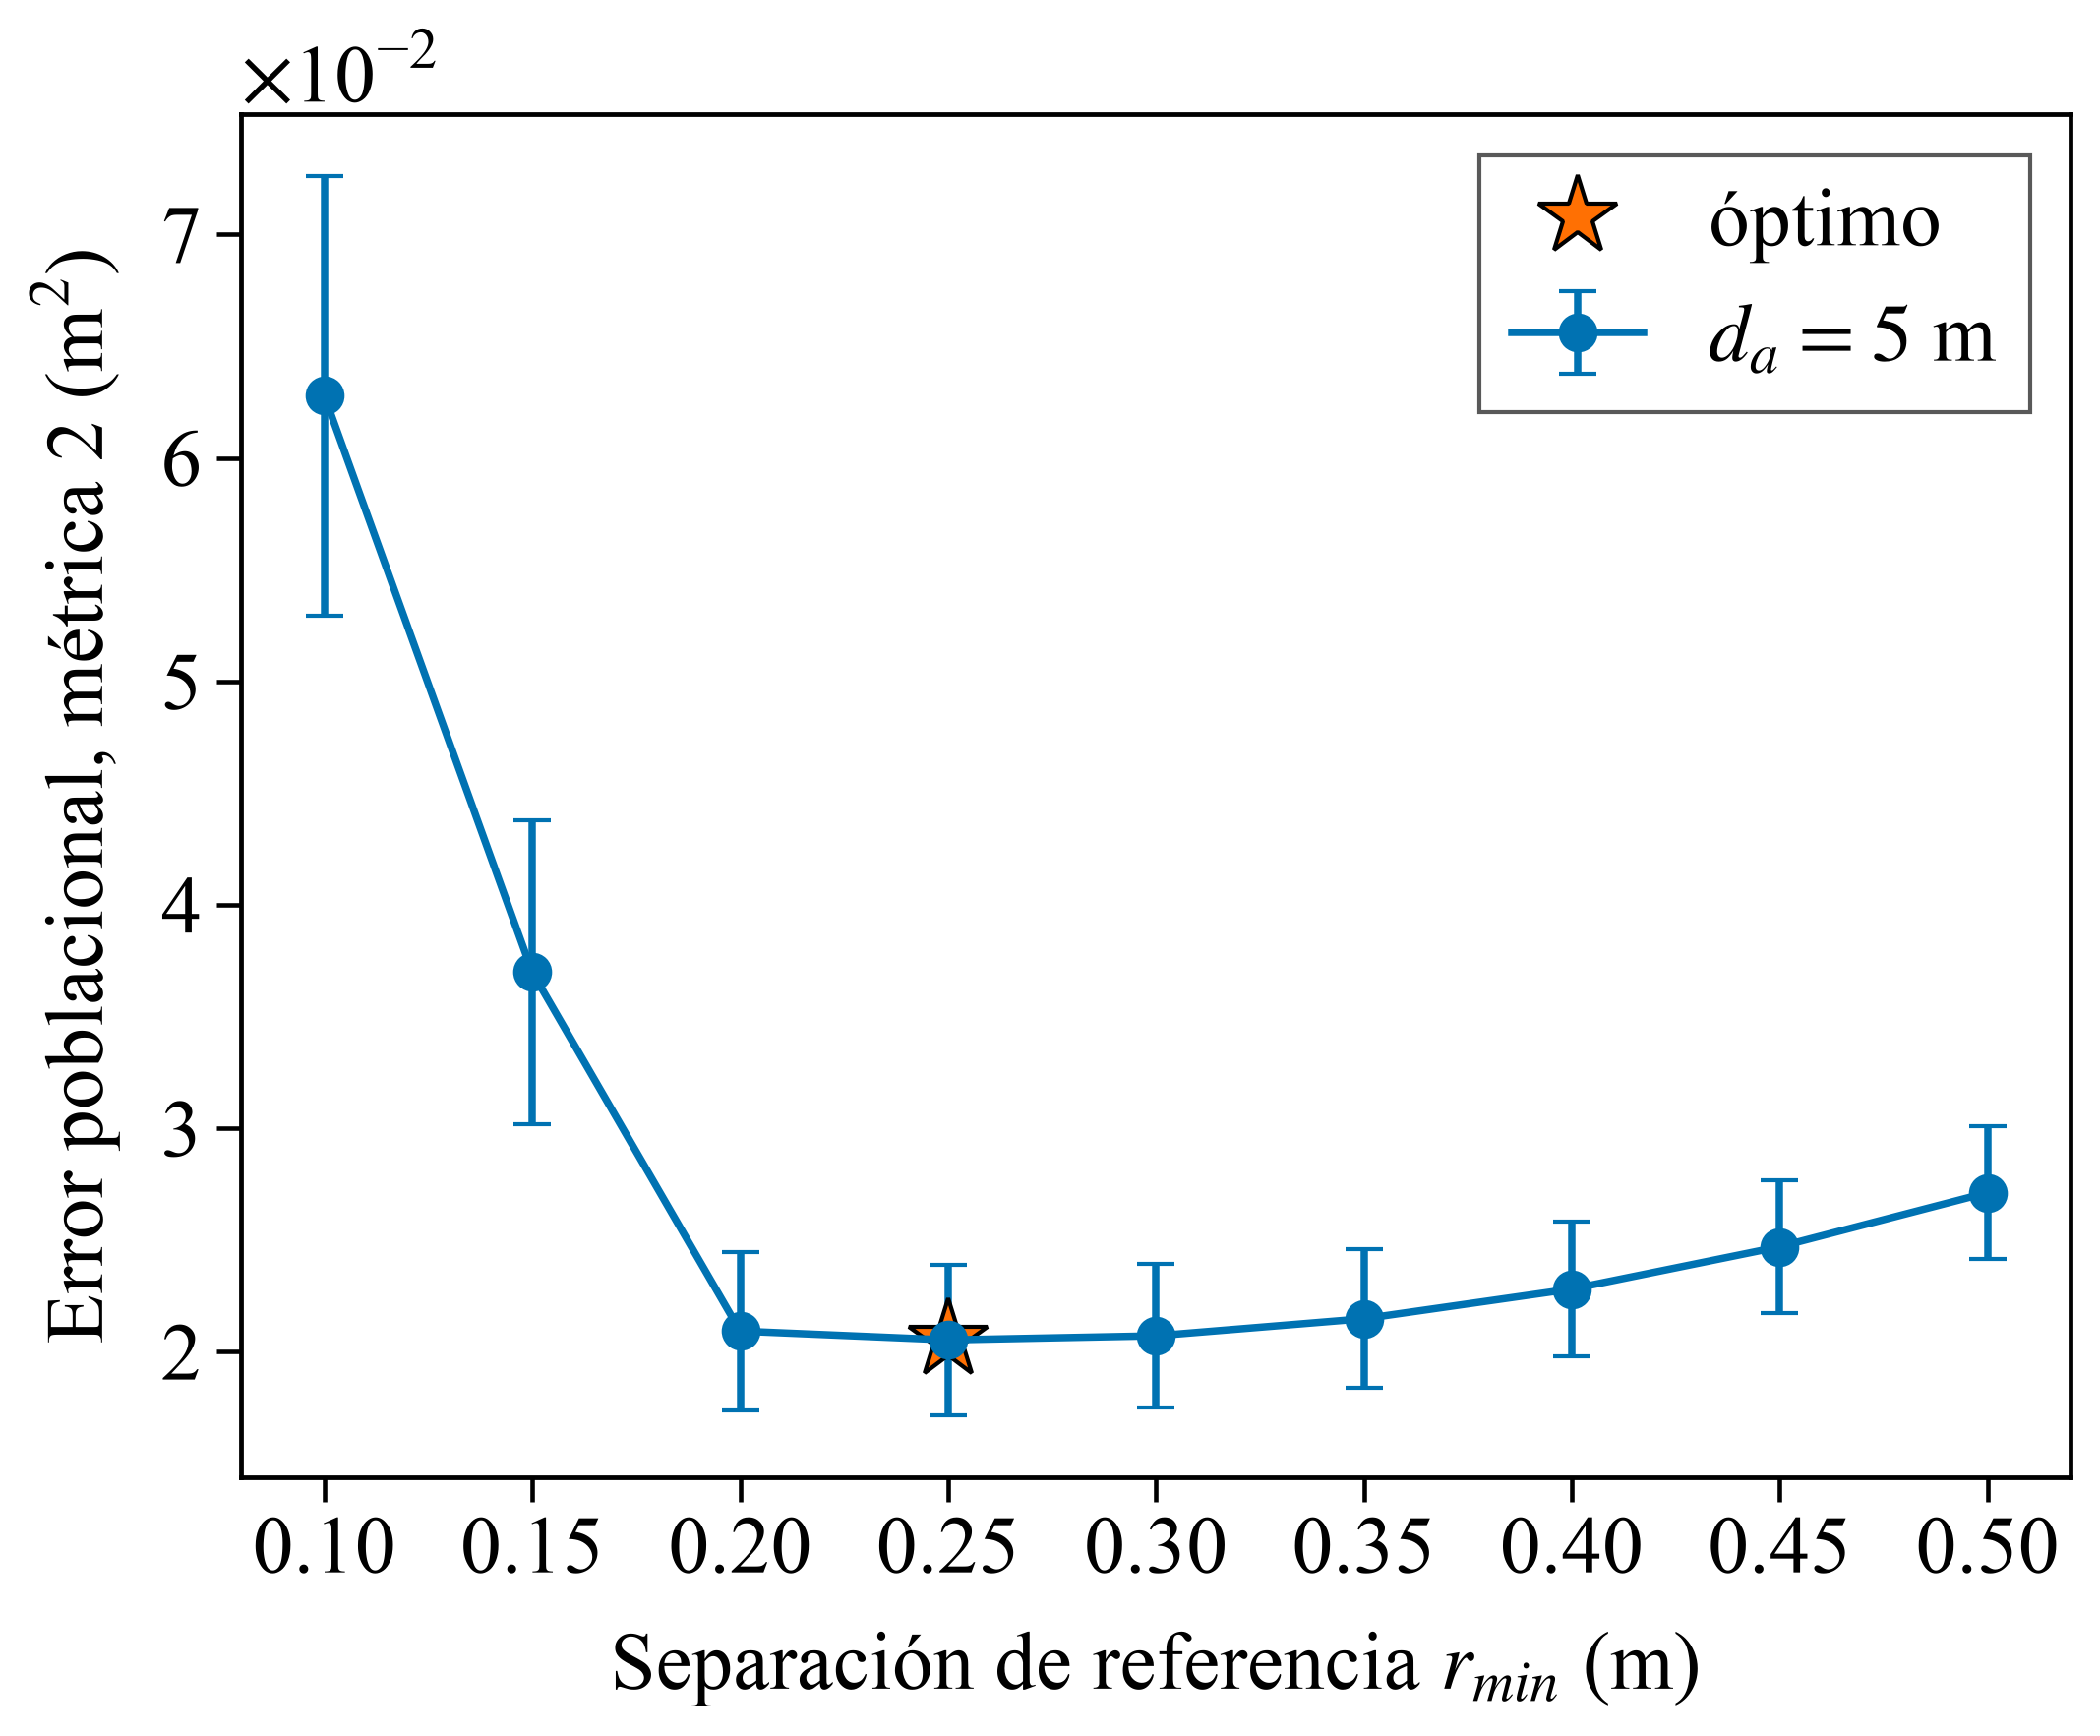
\includegraphics[width=\linewidth,height=0.62\textheight,keepaspectratio]{E2_corte_rmin.png}
    \end{column}
    \begin{column}{0.49\textwidth}
      \centering
      {\small Variando $\dact$, con $\dlat = 0.25\uni{m}$ fijo\par}
      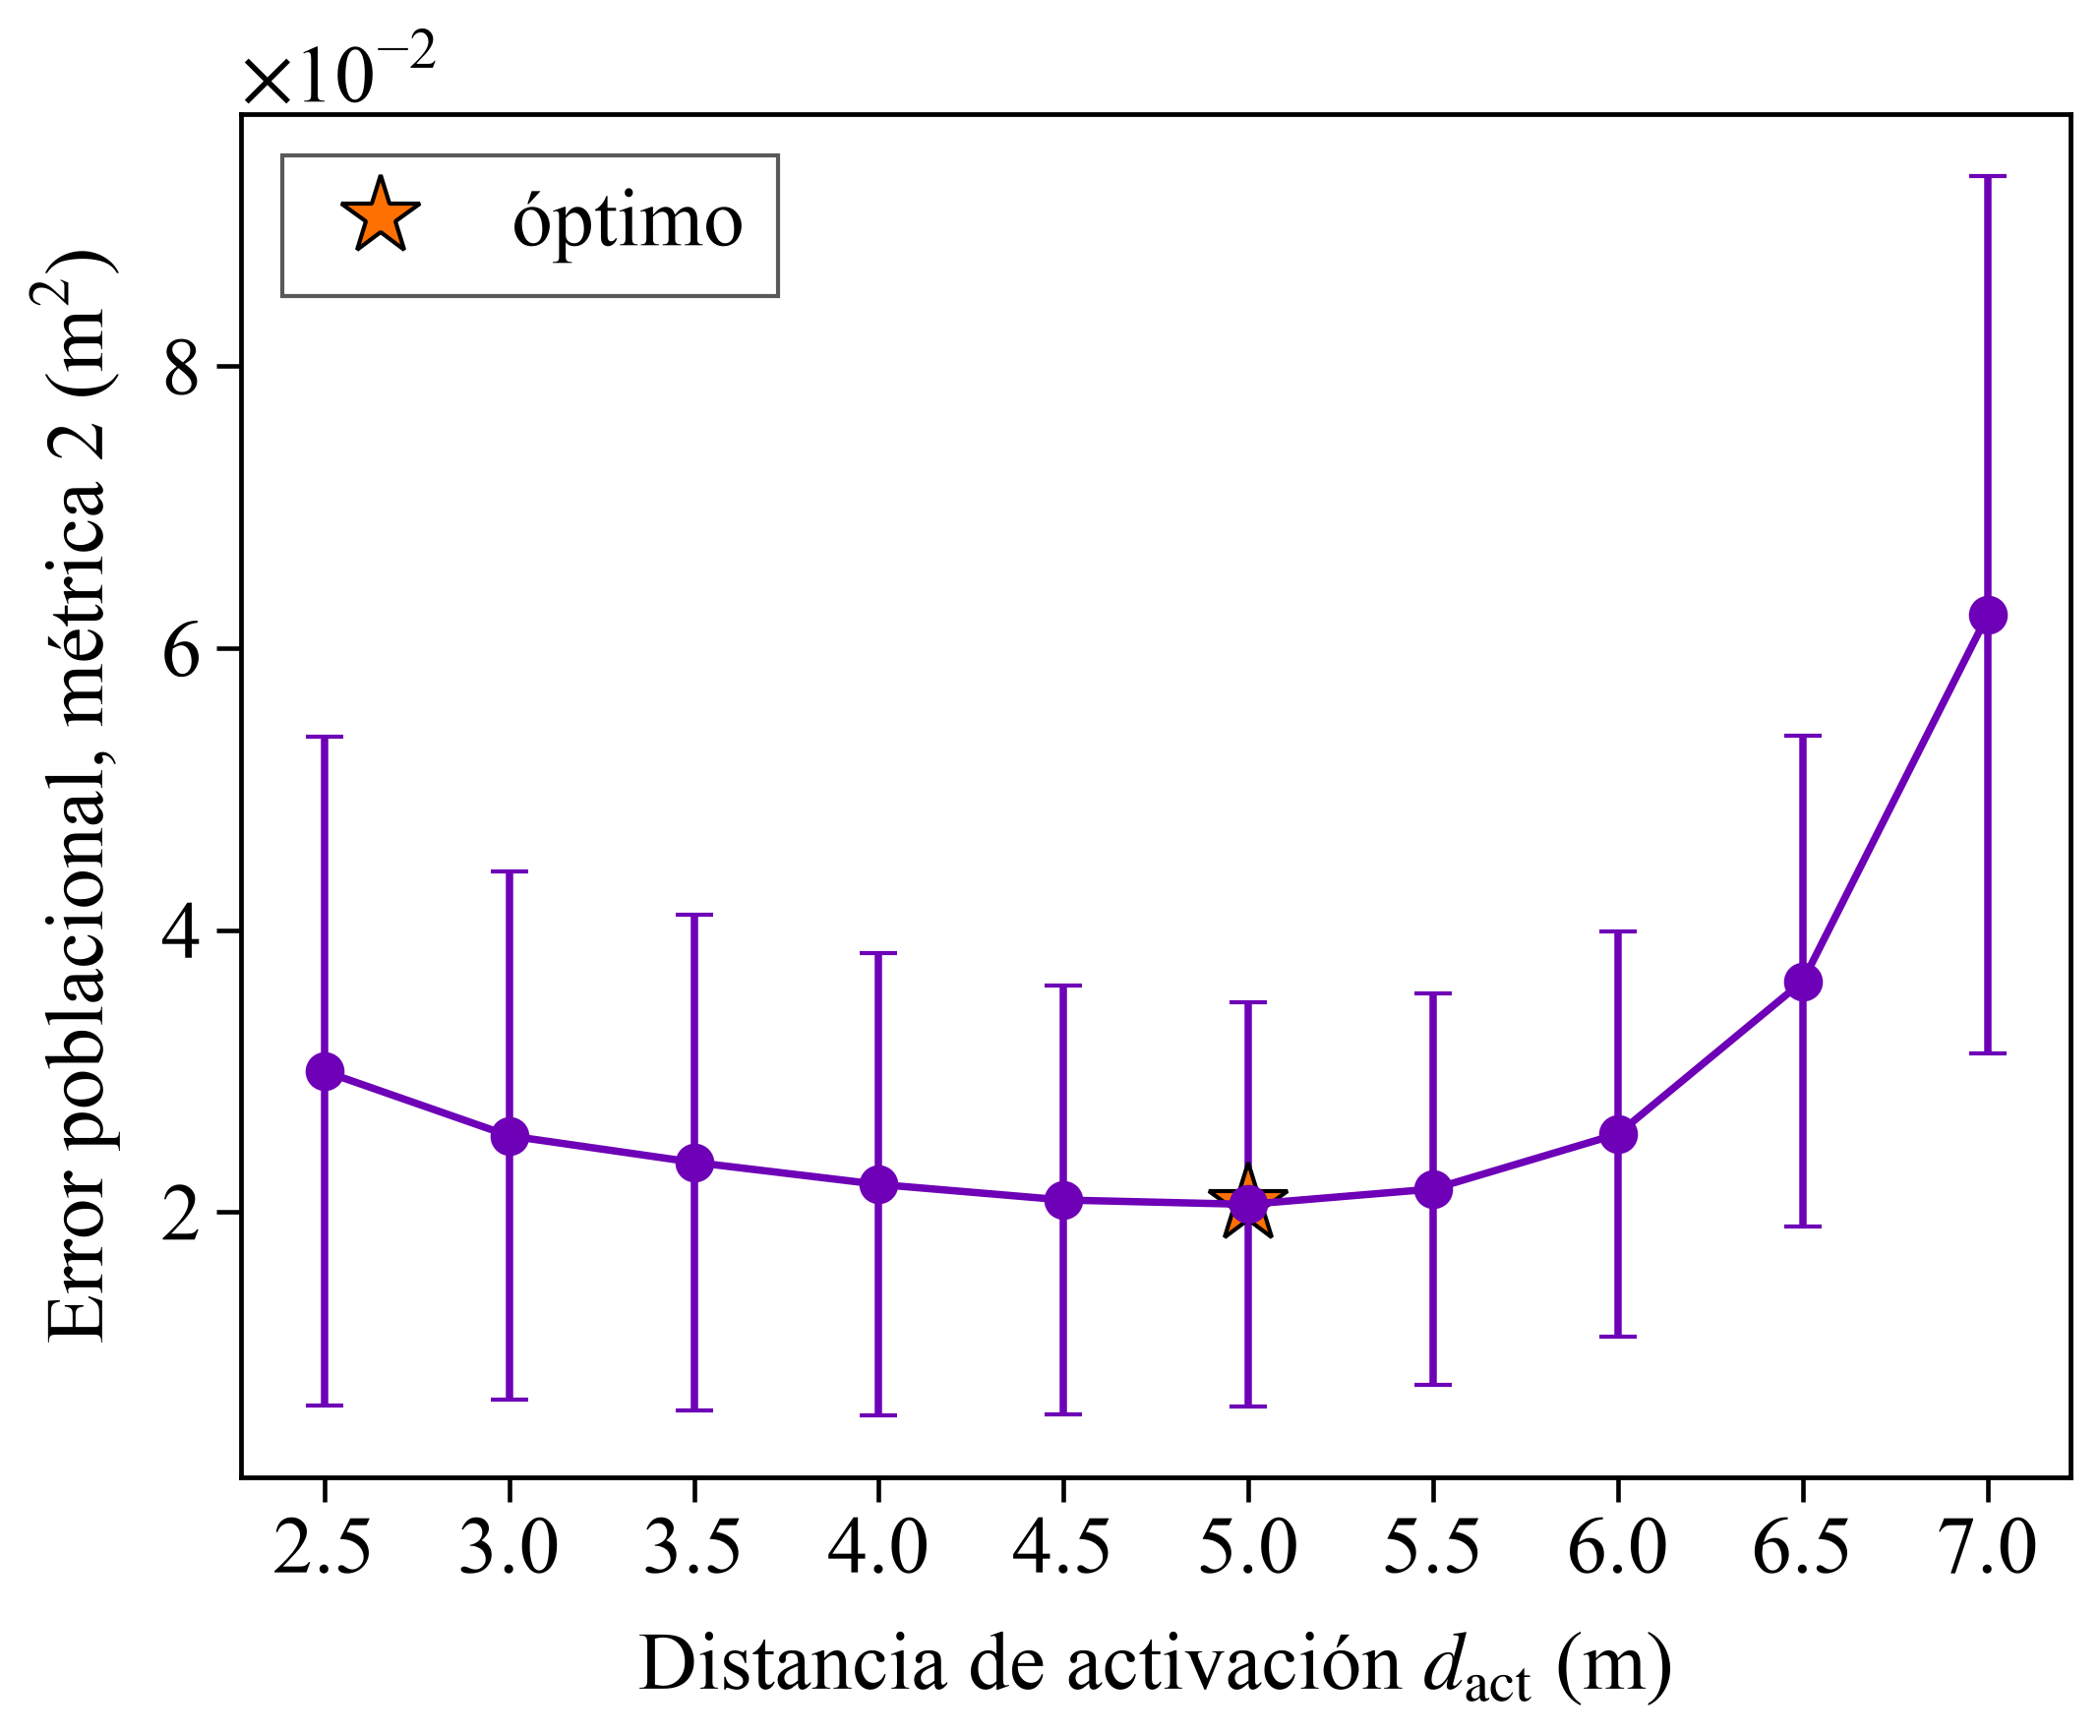
\includegraphics[width=\linewidth,height=0.62\textheight,keepaspectratio]{E2_corte_action_distance.png}
    \end{column}
  \end{columns}
\end{frame}

\begin{frame}{Resultados}
  \framesubtitle{Calibración poblacional: comparación de los óptimos}
  \centering
  \renewcommand{\arraystretch}{1.5}
  \begin{tabular}{lccc}
    \hline
    Métrica & $\dlat$ (m) & $\dact$ (m) & $\langle E\rangle$ (m$^2$) \\
    \hline
    1: iguales tiempos & $0.20$ & $4$ & $0.4 \pm 0.3$ \\
    2: punto más cercano & $0.25$ & $5$ & $(2 \pm 1)\ten{-2}$ \\
    \hline
  \end{tabular}

  \vspace{16pt}
  \begin{columns}
    \begin{column}{0.62\textwidth}
      \begin{resultado}
        \item Óptimos a un paso de grilla entre sí
        \item $\langle E^{(1)}\rangle \approx 19\,\langle E^{(2)}\rangle$
        \item $\sqrt{\langle E\rangle}$: $0.62\uni{m}$ (métrica 1), $0.14\uni{m}$ (métrica 2)
      \end{resultado}
    \end{column}
  \end{columns}
\end{frame}

\begin{frame}{Resultados}
  \framesubtitle{Calibración individual: óptimos de cada evento}
  \begin{columns}[T]
    \begin{column}{0.49\textwidth}
      \centering{\small Métrica 1}\par
      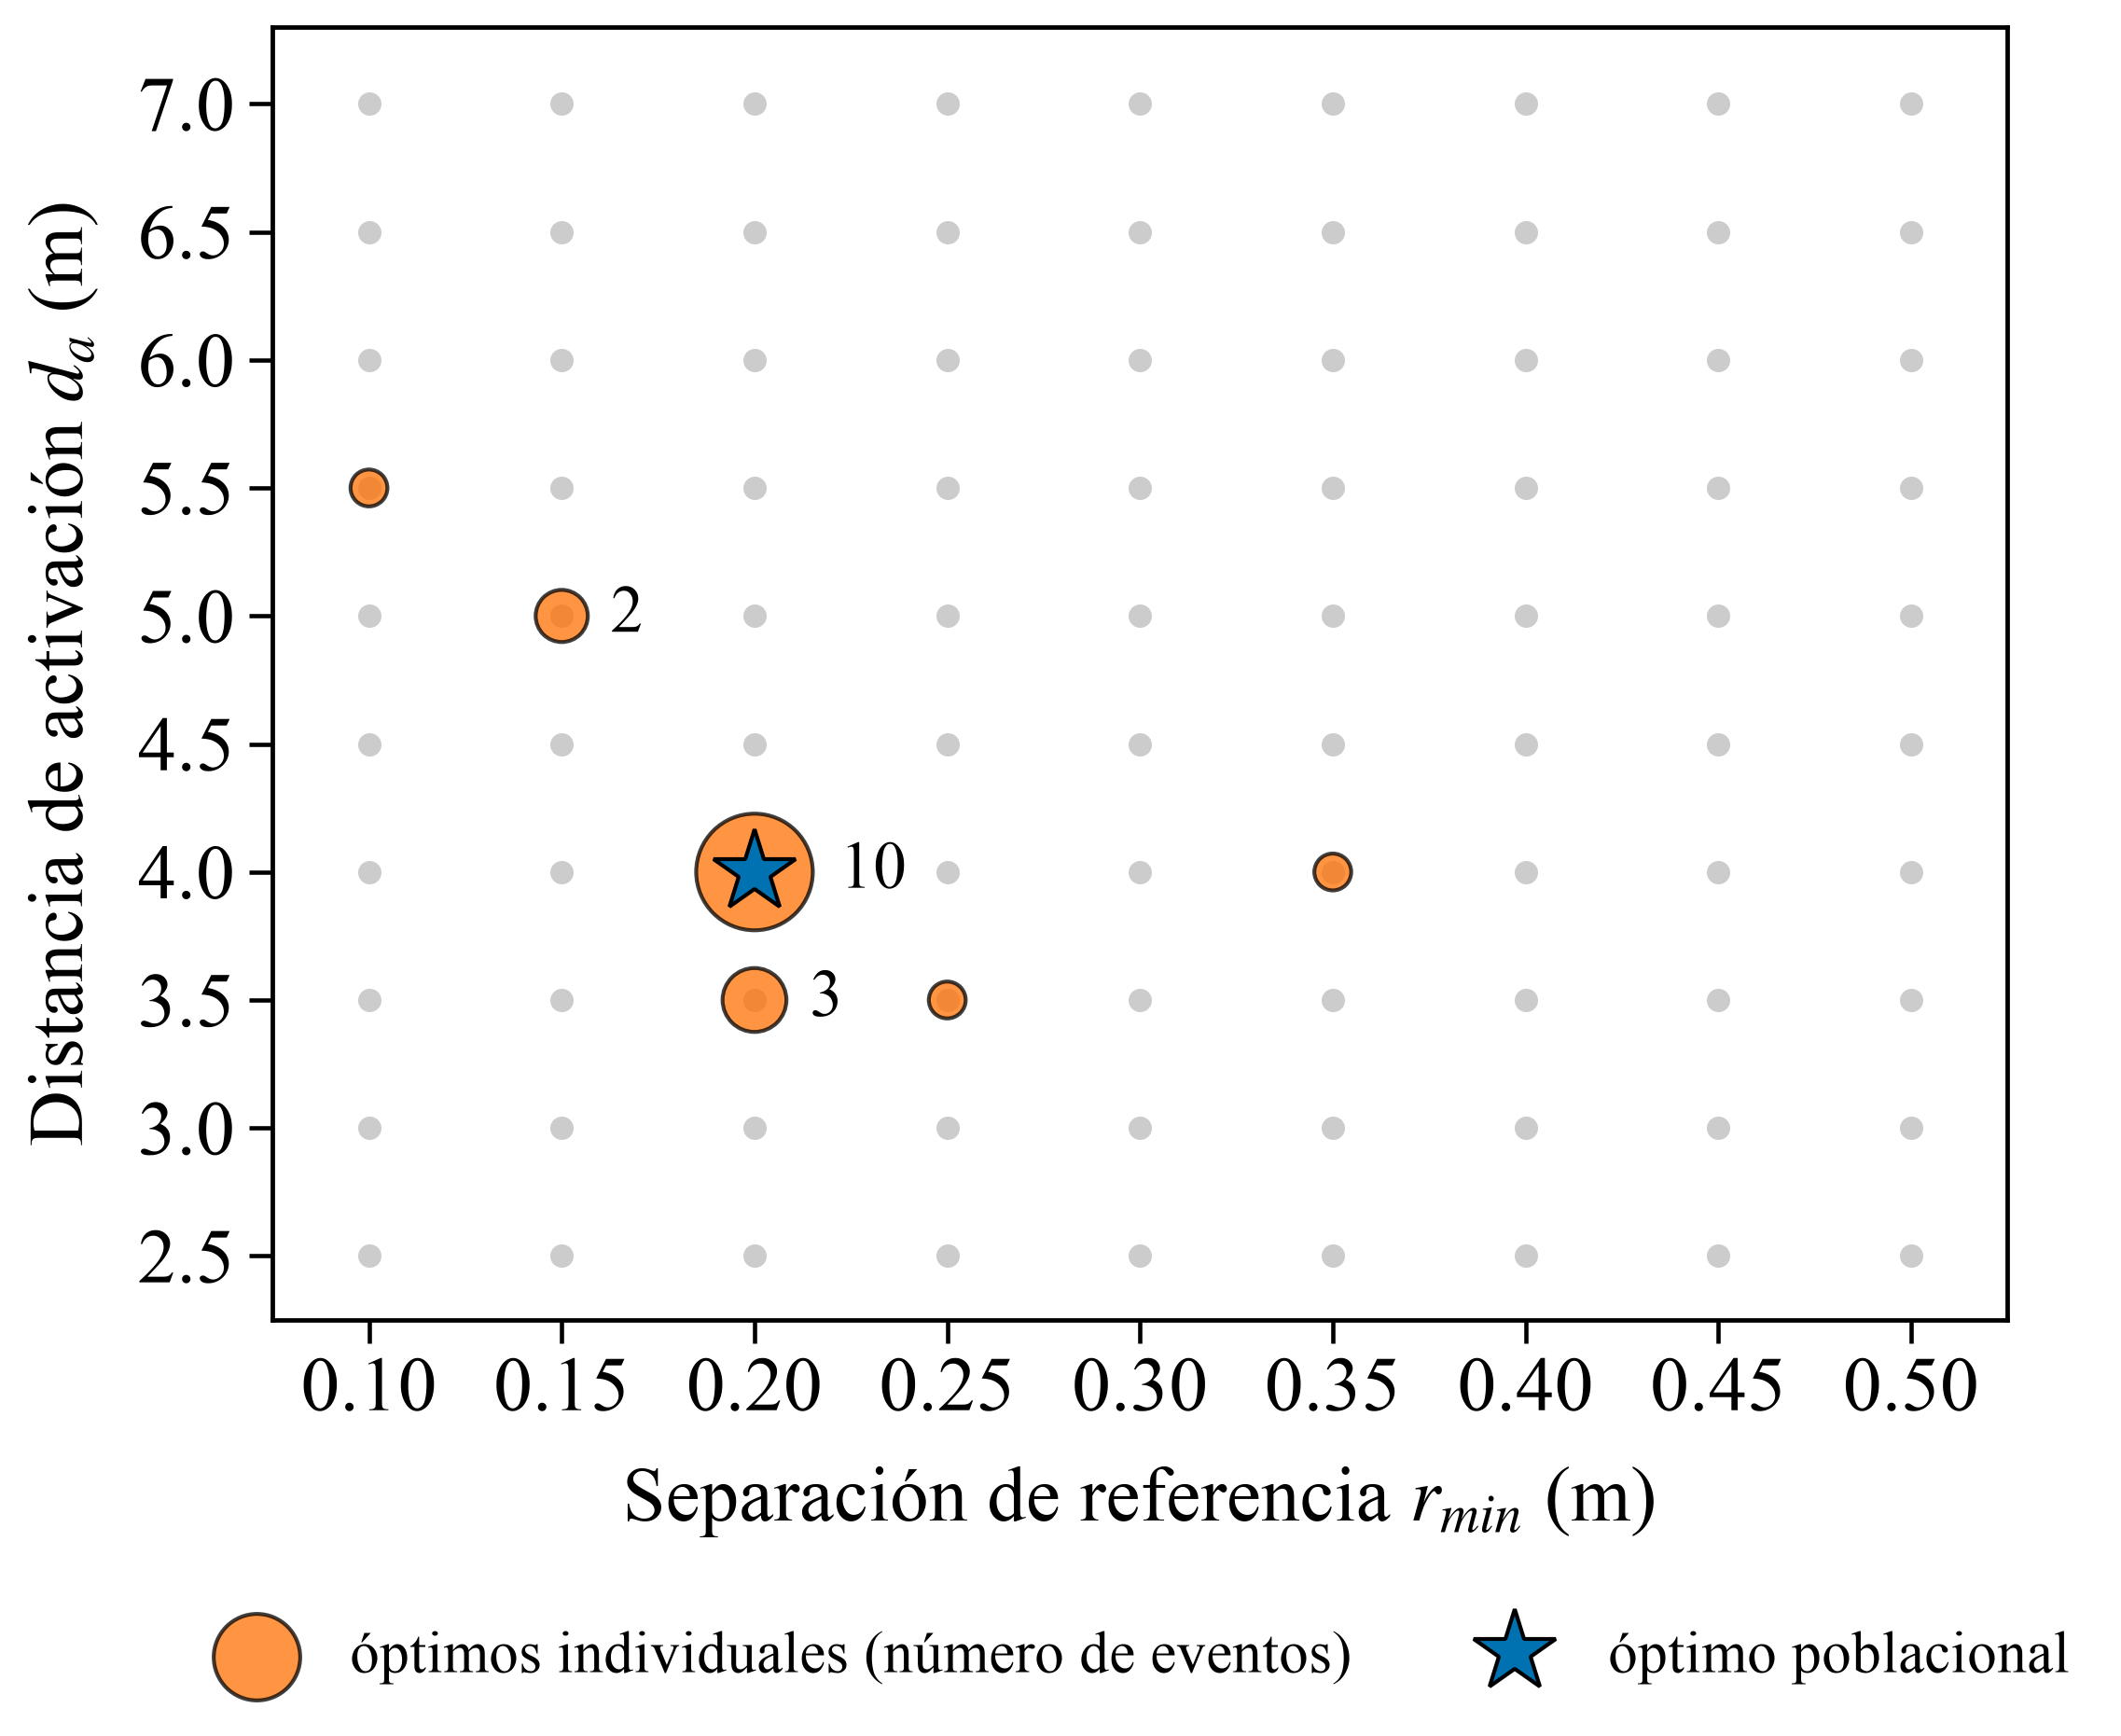
\includegraphics[width=\linewidth,height=0.70\textheight,keepaspectratio]{E1_optimos_individuales.png}
    \end{column}
    \begin{column}{0.49\textwidth}
      \centering{\small Métrica 2}\par
      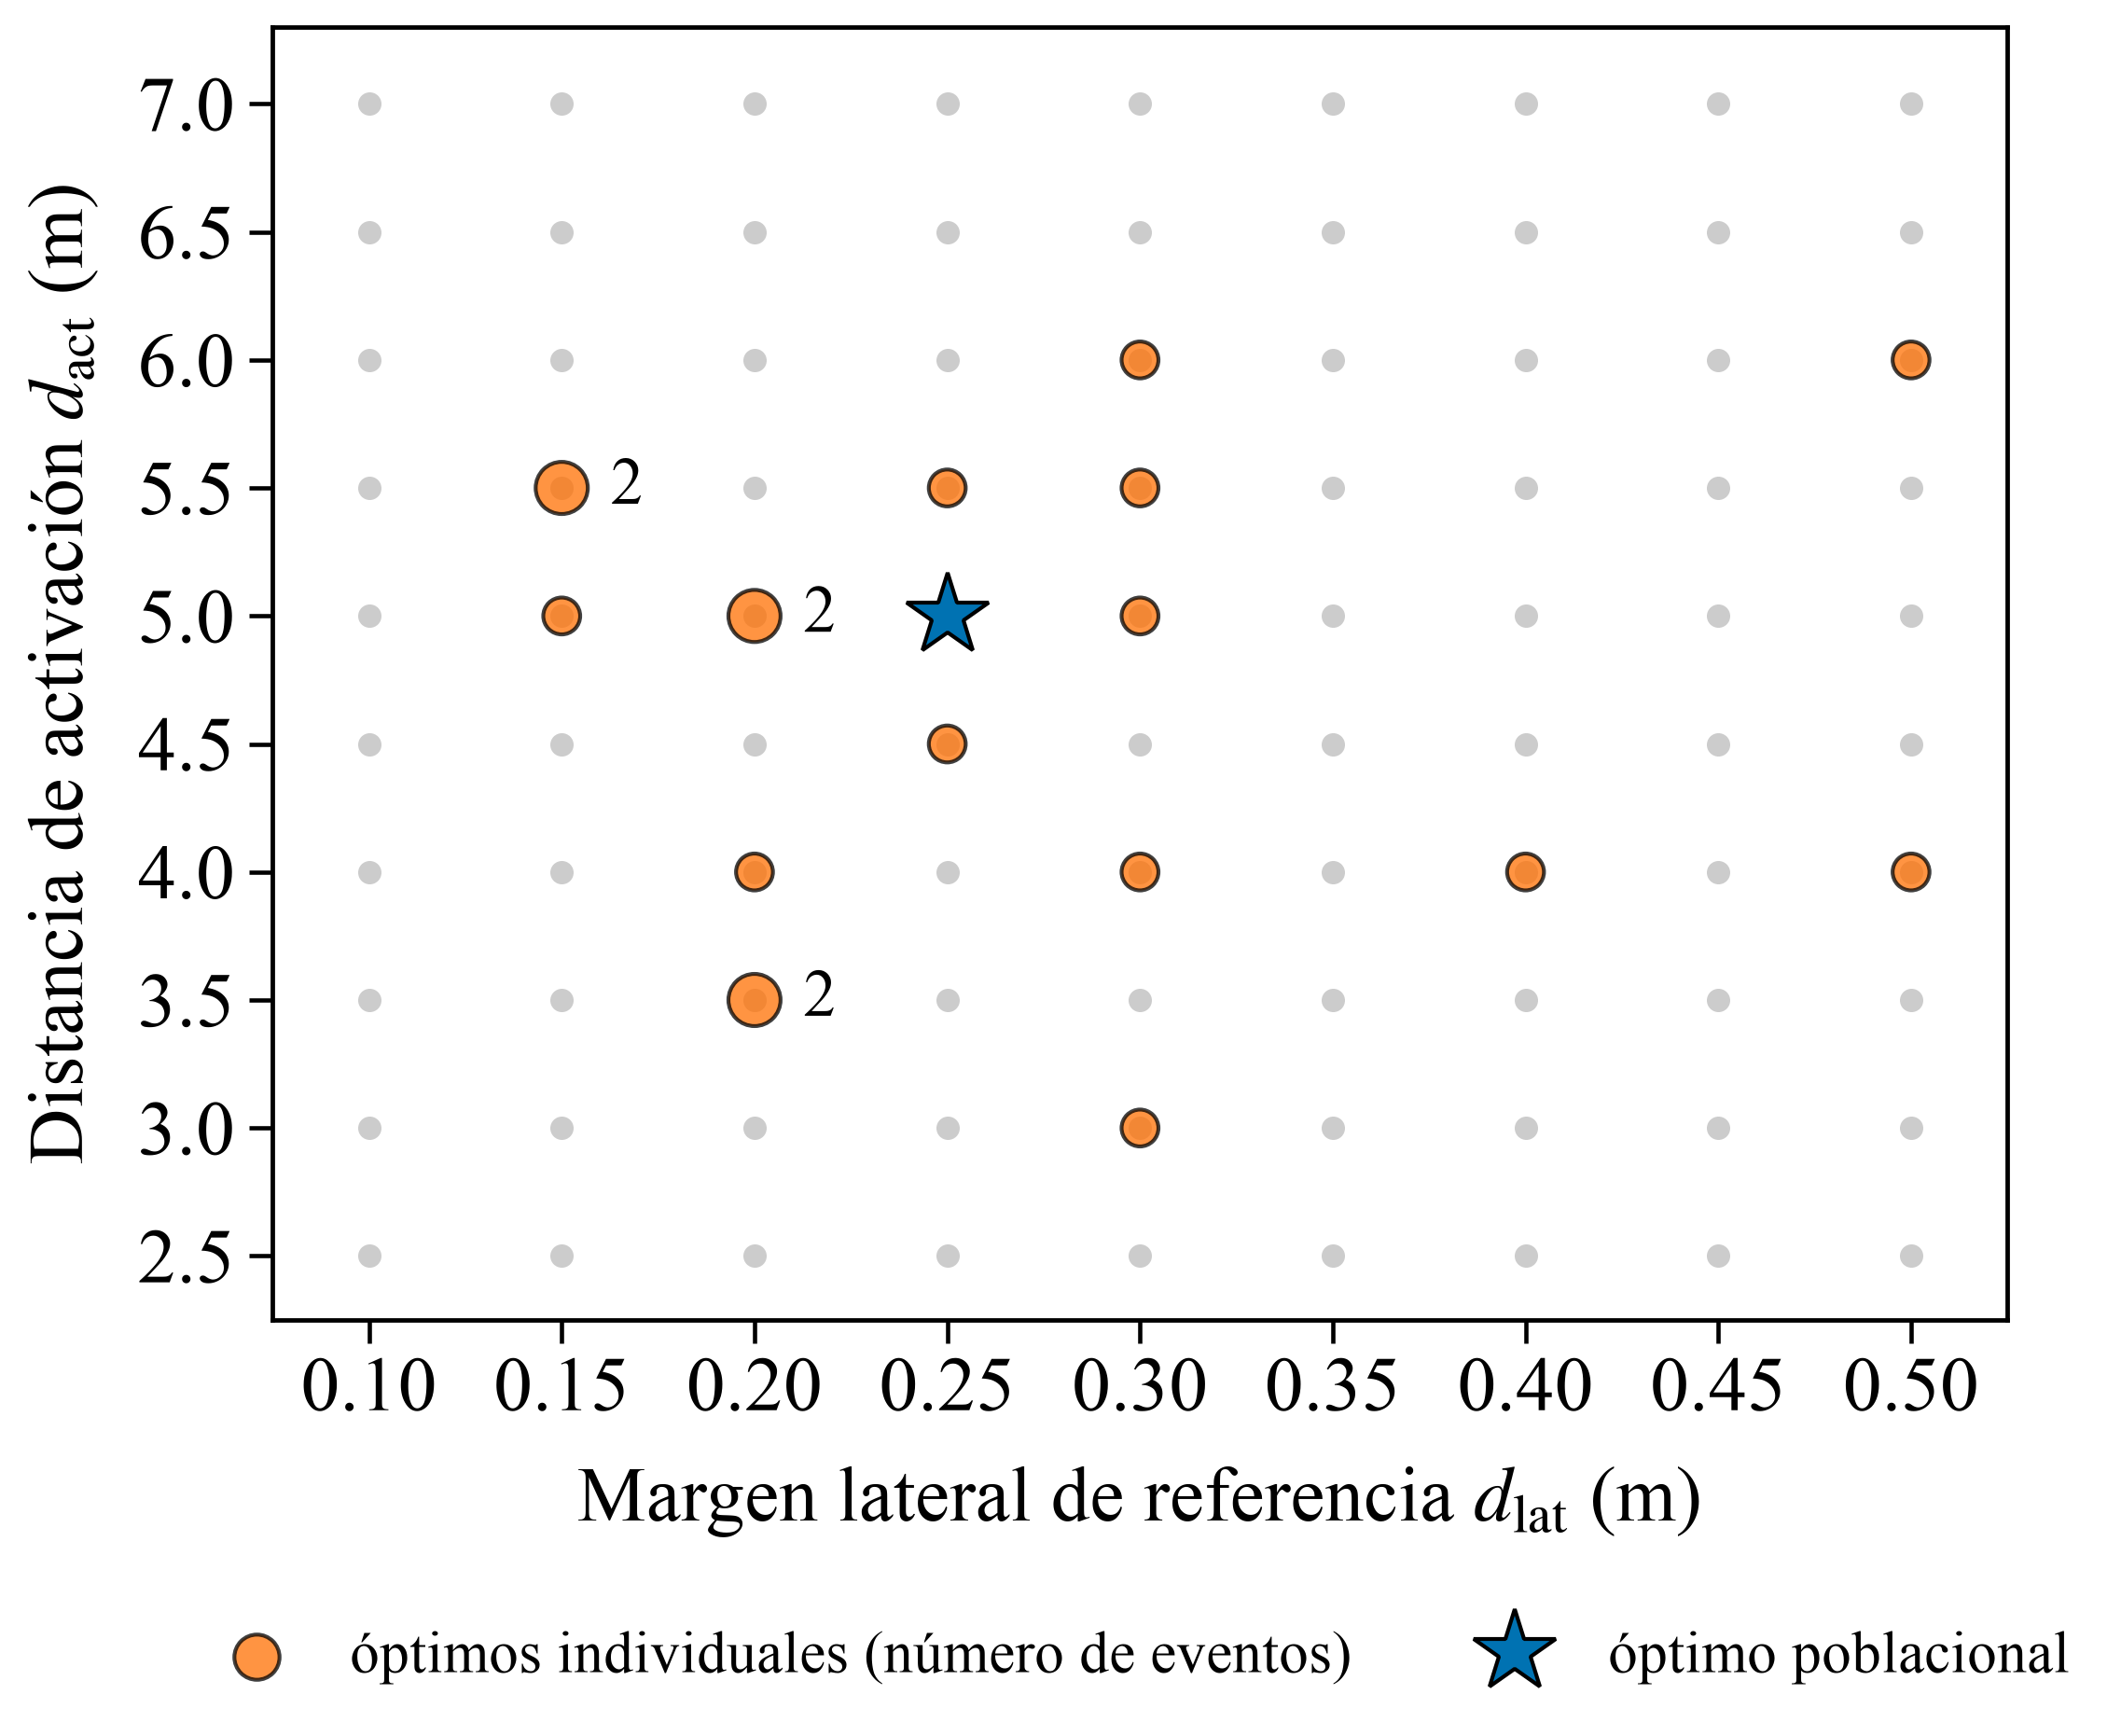
\includegraphics[width=\linewidth,height=0.70\textheight,keepaspectratio]{E2_optimos_individuales.png}
    \end{column}
  \end{columns}
\end{frame}

\begin{frame}{Resultados}
  \framesubtitle{Calibración individual: error de cada evento}
  \begin{columns}[T]
    \begin{column}{0.49\textwidth}
      \centering{\small Métrica 1}\par
      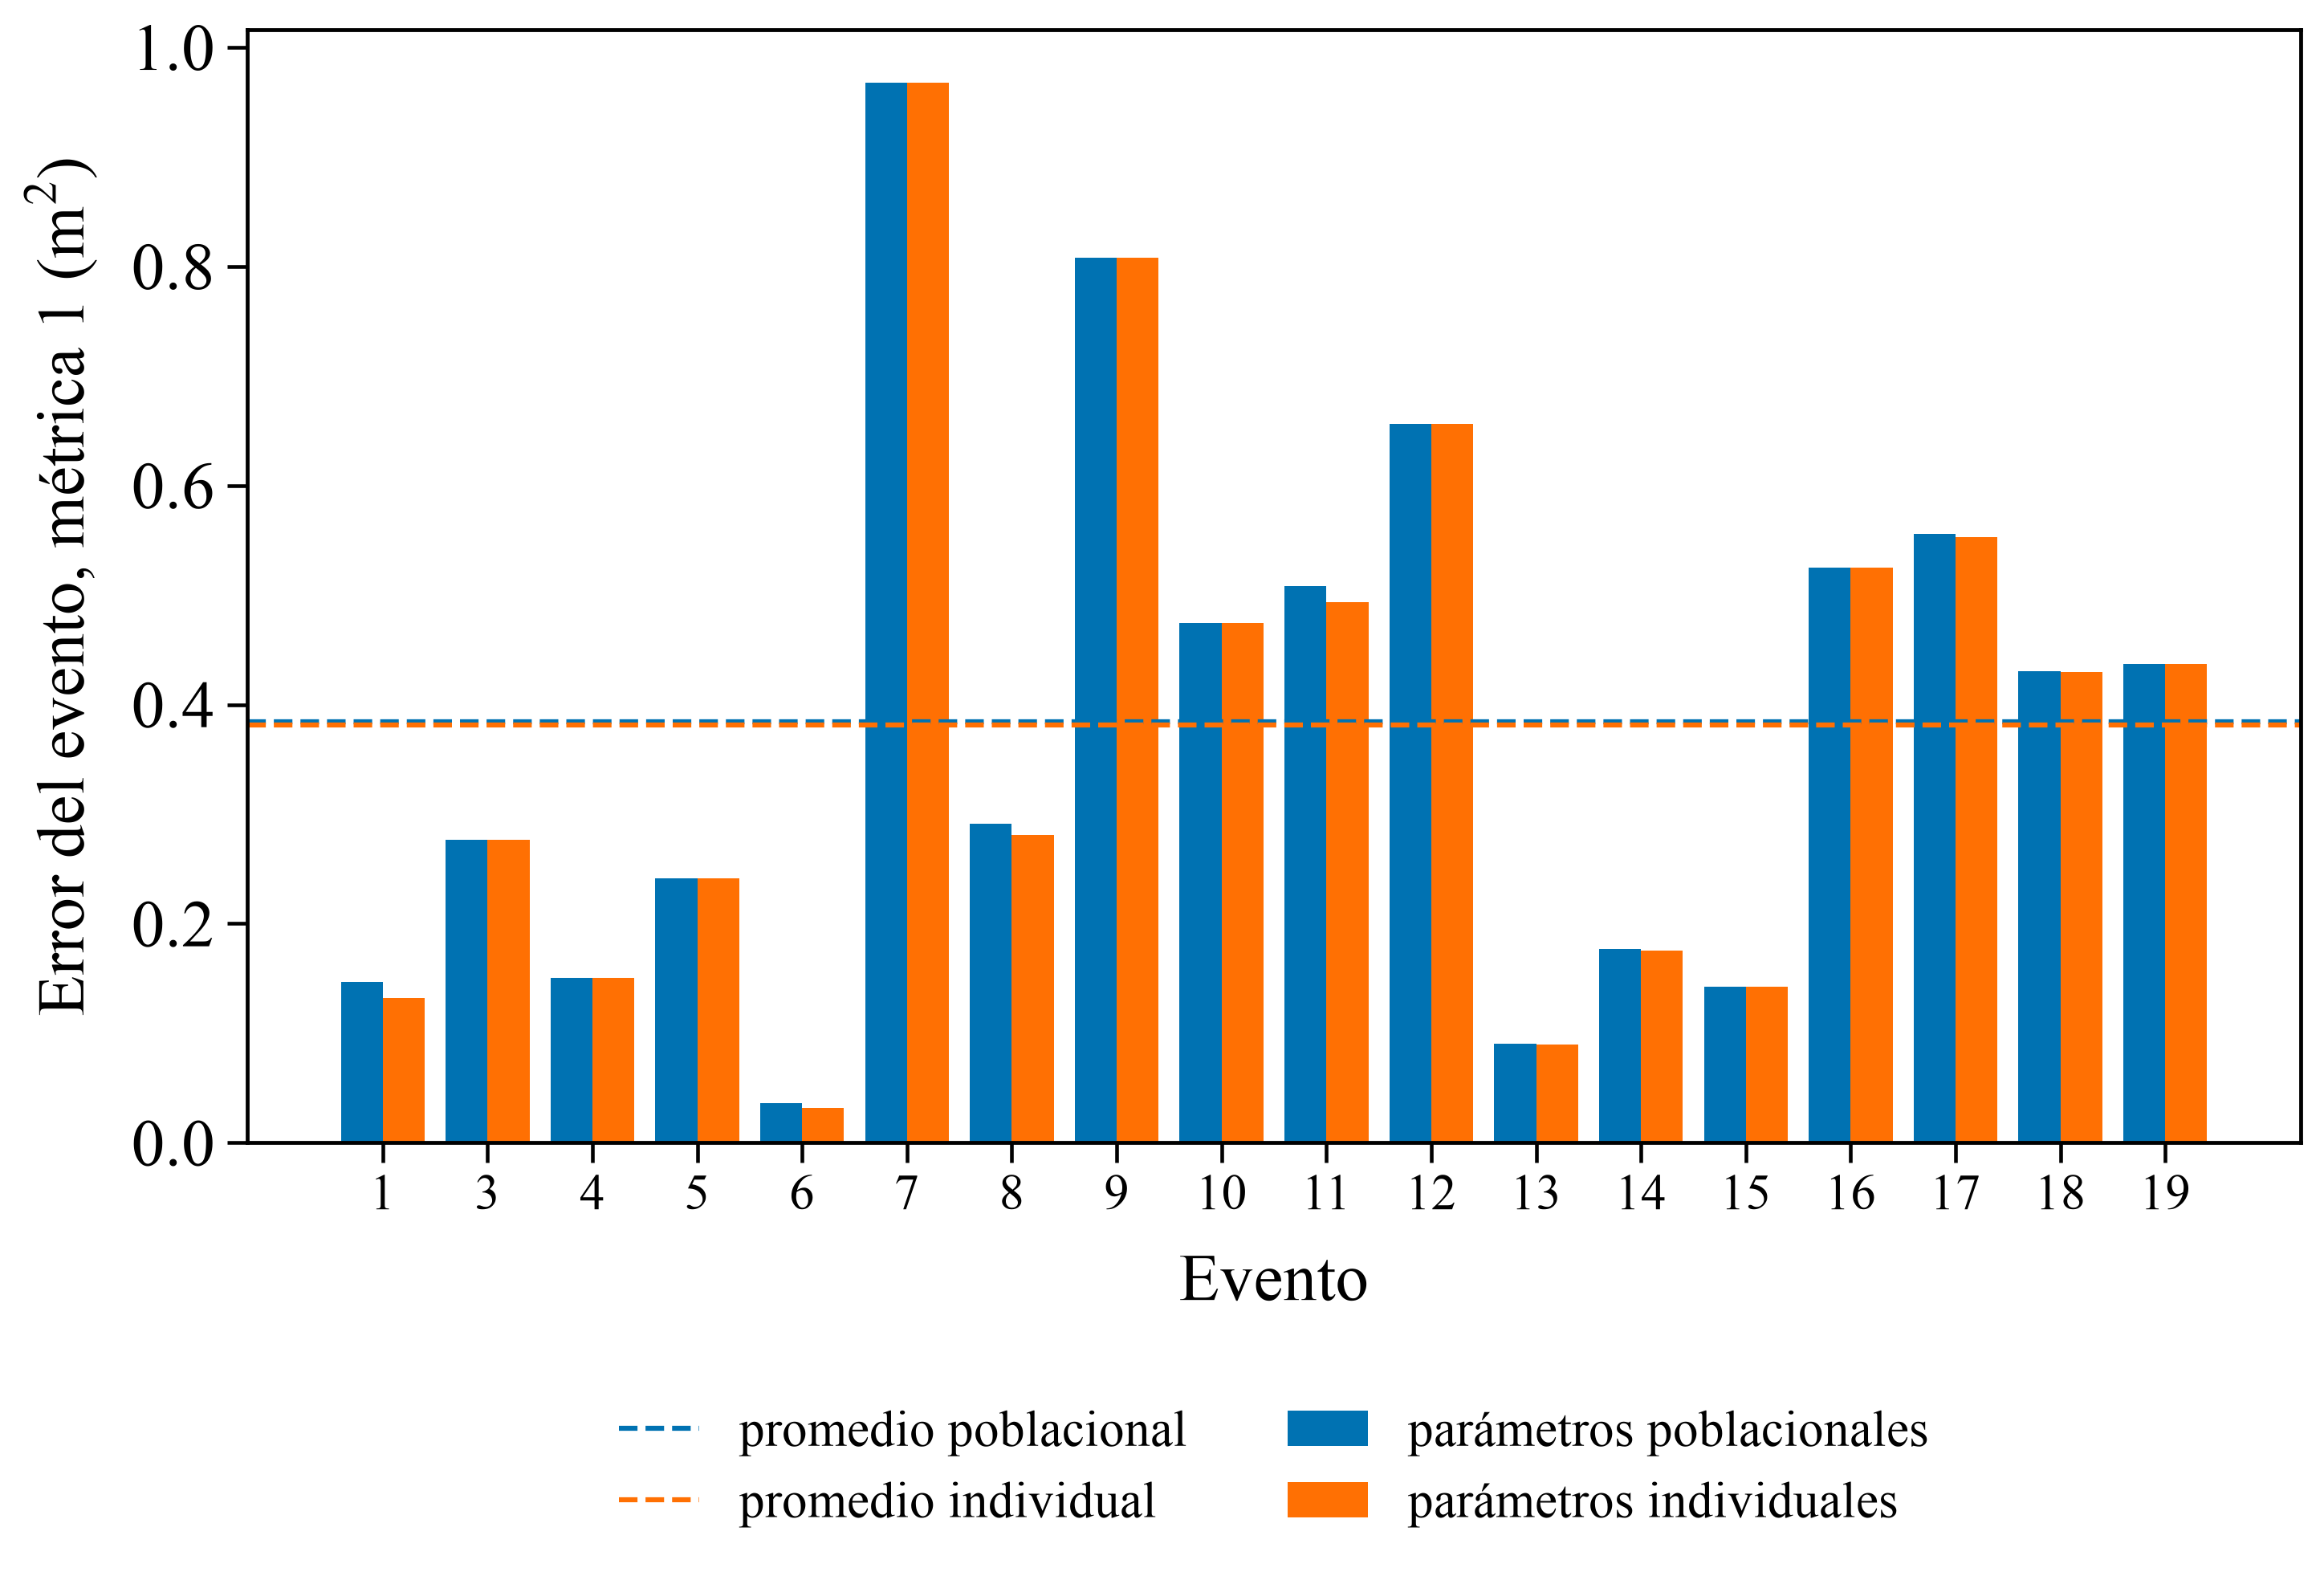
\includegraphics[width=\linewidth,height=0.70\textheight,keepaspectratio]{E1_error_por_evento.png}
    \end{column}
    \begin{column}{0.49\textwidth}
      \centering{\small Métrica 2}\par
      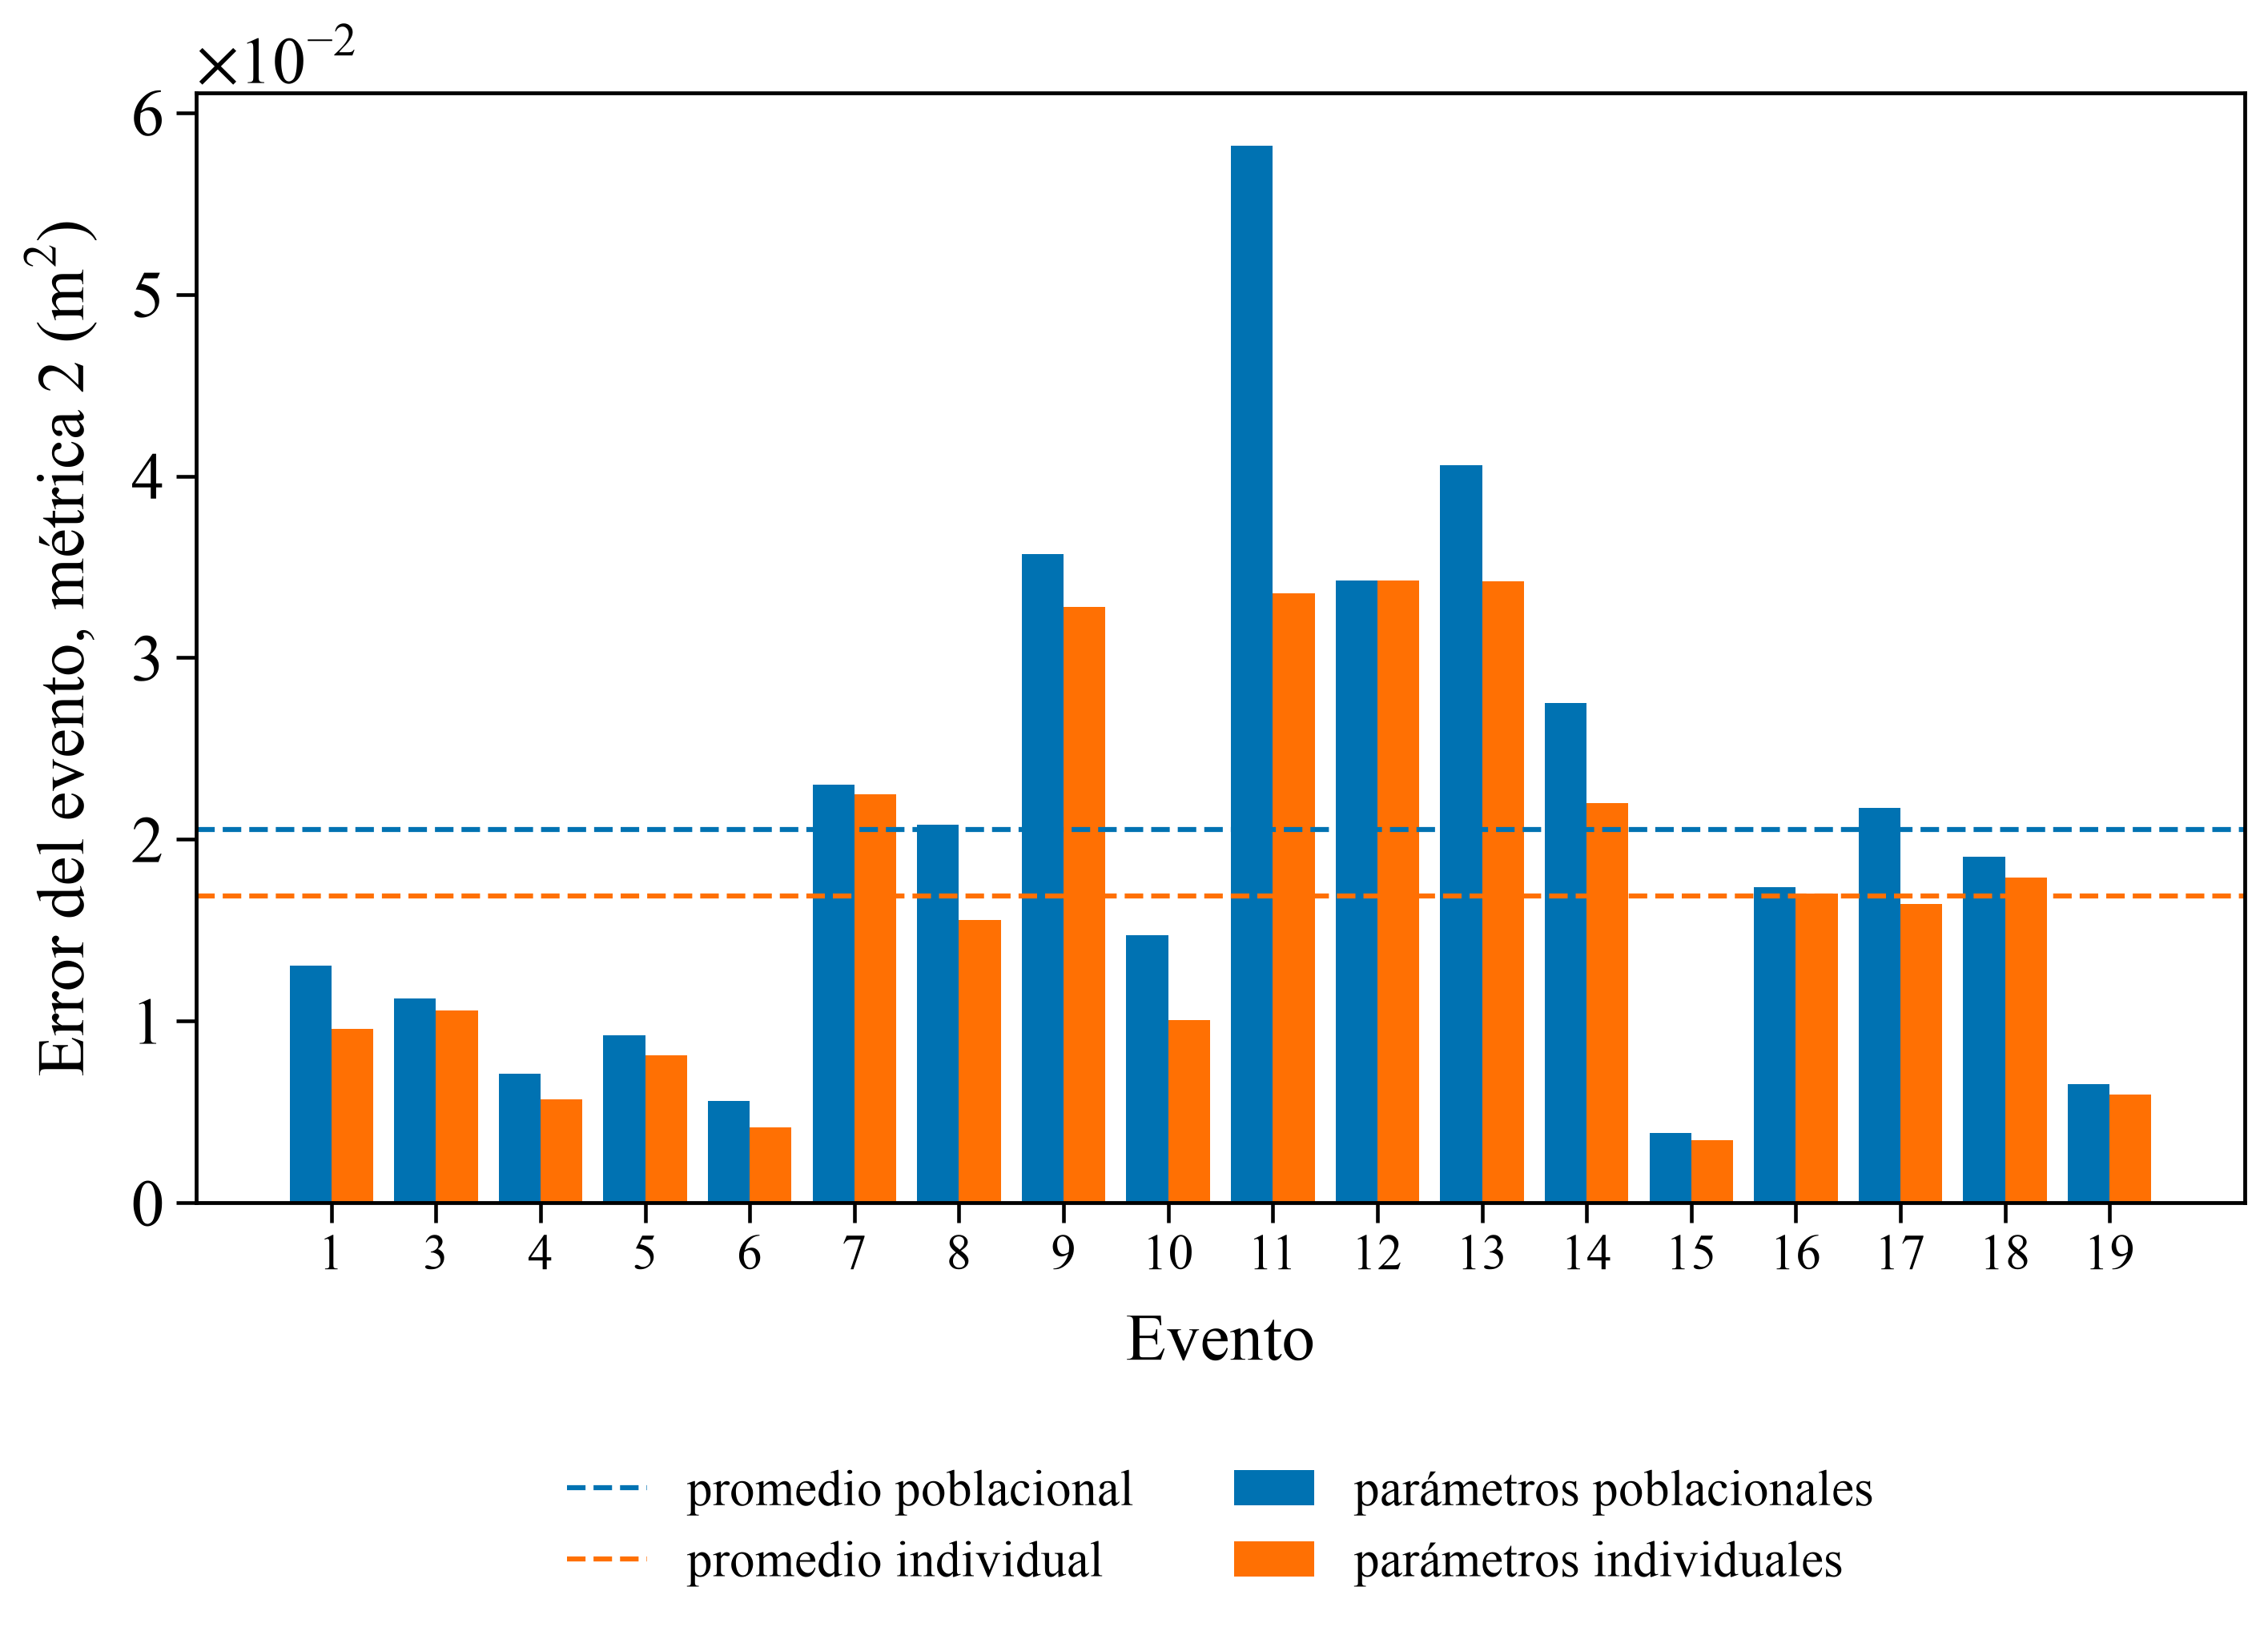
\includegraphics[width=\linewidth,height=0.70\textheight,keepaspectratio]{E2_error_por_evento.png}
    \end{column}
  \end{columns}
\end{frame}

\begin{frame}{Resultados}
  \framesubtitle{Calibración individual: ganancia al individualizar}
  \centering
  \renewcommand{\arraystretch}{1.5}
  \begin{tabular}{lccc}
    \hline
    Métrica & $\langle E\rangle$ poblacional (m$^2$) & $\langle E\rangle$ individual (m$^2$) & Ganancia \\
    \hline
    1: iguales tiempos & $0.384$ & $0.381$ & $0.7$\,\% \\
    2: punto más cercano & $2.05\ten{-2}$ & $1.69\ten{-2}$ & $18$\,\% \\
    \hline
  \end{tabular}

  \vspace{16pt}
  \begin{columns}
    \begin{column}{0.62\textwidth}
      \begin{resultado}
        \item Ganancia $= \big(\langle E\rangle_{\mathrm{pob}} - \langle E\rangle_{\mathrm{ind}}\big) / \langle E\rangle_{\mathrm{pob}}$
        \item $\sqrt{\langle E\rangle}$, métrica 1: $0.620 \to 0.618\uni{m}$
        \item $\sqrt{\langle E\rangle}$, métrica 2: $0.143 \to 0.130\uni{m}$
      \end{resultado}
    \end{column}
  \end{columns}
\end{frame}

\begin{frame}{Resultados}
  \framesubtitle{Validación cruzada}
\end{frame}
